%--------------A VOTRE ATTENTION-------------%
% Gabarit officiel IFRI (Licence) : New IFRI template latex 05-04-2020.
% Fichier principal (anciennement main.tex), renommé pour produire build/memoire.pdf.
% Les Membres doivent figurer dans la dernière version finale du mémoire après soutenance pour dépôt de mémoire

\documentclass{ifri}
\usepackage{titletoc}
\usepackage{tabularx}
\usepackage{booktabs}
\usepackage{tikz}
\usetikzlibrary{arrows.meta}
\usetikzlibrary{shapes.multipart}
% --- Macros de schémas UML ---
\newcommand{\acteur}[3]{\begin{scope}[shift={(#2)}]\draw (0,0.35) circle (0.14);\draw (0,0.21)--(0,-0.2);\draw (-0.25,0.05)--(0.25,0.05);\draw (0,-0.2)--(-0.2,-0.55);\draw (0,-0.2)--(0.2,-0.55);\node[font=\scriptsize, align=center, below] at (0,-0.55) {#3};\coordinate (#1) at (0,0);\end{scope}}
\newcommand{\seqhead}[3]{\node[draw, font=\scriptsize, align=center, minimum width=2.1cm, minimum height=0.7cm, fill=gray!10] (#1) at (#2,0) {#3};}
\newcommand{\seqlife}[2]{\draw[gray, dashed] (#1.south) -- (#1 |- 0,#2);}
\newcommand{\seqmsg}[5]{\draw[->, #5] (#1,#3) -- node[above, font=\tiny, align=center, inner sep=1pt] {#4} (#2,#3);}
\newcommand{\seqself}[4]{\draw[->] (#1,#2) -- ++(0.6,0) -- ++(0,-0.45) -- ++(-0.6,0); \node[right, font=\tiny, align=left, text width=#4, inner sep=1pt, anchor=north west] at (#1+0.65,#2+0.05) {#3};}
% Emplacement d'image : affiche l'image si le fichier existe, sinon un cadre rouge à compléter
\newcommand{\imageouplace}[4]{\begin{figure}[H]\centering\IfFileExists{images/#1}{\includegraphics[width=#2]{images/#1}}{\fbox{\parbox{#2}{\centering\vspace{1.4cm}\textcolor{red}{\textbf{[Image à fournir : #3]}}\vspace{1.4cm}}}}\caption{#3}\label{#4}\end{figure}}
\setlength{\glsdescwidth}{0.65\textwidth}
\setlength{\emergencystretch}{2em}
% \usepackage{lscape}

% --- Marqueurs de travail (en rouge dans le PDF tant qu'ils ne sont pas traités) ---
\newcommand{\asourcer}{\textcolor{red}{\textbf{[SOURCE À FOURNIR]}}}
\newcommand{\adonner}[1]{\textcolor{red}{\textbf{[#1]}}}
\newcommand{\aredigerr}{\par\noindent\textcolor{gray}{\emph{À rédiger.}}\par}

\addto\captionsfrench{\renewcommand{\listfigurename}{Liste des figures}\renewcommand{\listtablename}{Liste des tableaux}}

\typeMemoire{Diplôme de Licence en Informatique}
\optionFormation{\adonner{Option à confirmer}}
\etudiant{Hugues \textbf{HANTAN}}
\titreDuMemoire{Conception et implémentation d'une infrastructure de contrôle d'accès biométrique intelligente par vision artificielle et architecture Edge Computing : le système BioGate} % À confirmer par l'étudiant

\dateSoutenance{-}
%\promo{2\up{ème}}
\anneeScolaire{\adonner{Année académique à confirmer}}


%%maitre de mémoire
\encadrants{\adonner{Grade à confirmer} Probus \textbf{KIKI}}

%% Membres du Jury
\jurys{%
\begin{tabular}{llll}
	\adonner{Nom du président} & \adonner{Grade} & \adonner{Entité} & Président \\
	\adonner{Nom de l'examinateur} & \adonner{Grade} & \adonner{Entité} & Examinateur \\
	\adonner{Nom du rapporteur} & \adonner{Grade} & \adonner{Entité} & Rapporteur \\
\end{tabular}
}


\hypersetup{
 pdftitle={Conception et implémentation d'une infrastructure de contrôle d'accès biométrique : BioGate},
 pdfauthor={Hugues HANTAN},
 pdfsubject={Mémoire de Licence en Informatique}
 }

\color{bookColor}

%importation du glossaire
\loadglsentries{glossaire_reduit}

\begin{document}

\pageDeGarde
%\pageTitre

\pagecolor{white}

%% page vide
%\thispagestyle{empty}\ \clearpage


\selectlanguage{french}

% sommaire
\pagenumbering{roman}

\setcounter{tocdepth}{0}
\startlist{toc}
\printlist{toc}{}{\chapter*{Sommaire}}
\setcounter{tocdepth}{5}

%% rdedicaces
\dedicace
\begin{nouv}
À ma famille, pour son amour, ses sacrifices et son soutien constant.
\end{nouv}

\newpage

%% remerciements
\remerciements

Je remercie ma famille pour son soutien constant tout au long de ma formation.

Je remercie mon maître de mémoire, Probus KIKI, pour son encadrement et ses conseils.

Je rends grâce à Dieu, qui m'a donné la force et la santé de mener ce travail à son terme.

\newpage

% Résume
\resume
\selectlanguage{french}
\vspace*{-6cm}
\begin{abstract}
\aredigerr
% Un paragraphe : contexte, problème, objectif, démarche, résultats (à rédiger une fois les chapitres validés).

\paragraph{}
\textbf{Mots clés}: \adonner{4 à 5 mots clés à fournir}
\end{abstract}

\newpage
\thispagestyle{empty}
\selectlanguage{english}
\addcontentsline{toc}{chapter}{Abstract}
\begin{abstract}

\textcolor{gray}{\emph{To be written.}}

\paragraph{}
\textbf{Key words}: \textcolor{red}{\textbf{[to be provided]}}
\end{abstract}

\selectlanguage{french} % ajouté : le résumé se termine en anglais
\newpage

%liste des figures
\listoffigures
\newpage

%liste des tableaux
\listoftables
\newpage

%liste des algo : retirée (aucun algorithme dans ce mémoire) ; réactiver si besoin
%\selectlanguage{french}
%\listofalgorithmes
%\newpage

% Les sigles et acronymes
\setglossarystyle{altlist}
\printglossary[title=Liste des acronymes, toctitle=Liste des acronymes, type=\acronymtype]
\newpage

% Le glossaire proprement dit
\setglossarystyle{altlist}
\printglossary[type=main]


\pagenumbering{arabic}
\setcounter{page}{1}
%%introduction
\introduction
\markboth{Introduction générale}{Introduction générale}

Le contrôle d'accès vise à réserver l'entrée d'un lieu aux personnes autorisées. Il repose classiquement sur un objet détenu, tel qu'une clé ou un badge, ou sur un secret, tel qu'un code. Ces facteurs authentifient la possession d'un objet ou la connaissance d'une information, et non la personne elle-même : ils peuvent être copiés, prêtés, perdus ou observés. Les systèmes à badge ou à code conservent un historique des passages, mais celui-ci identifie le badge ou le code utilisé, et non son porteur.

La biométrie remplace ces facteurs par une caractéristique propre à l'individu. La reconnaissance faciale a pour avantage de s'effectuer sans contact, à partir d'une simple caméra. Elle repose cependant sur une comparaison statistique dont le résultat est une mesure de ressemblance et non une certitude. La décision d'accès est donc prise sous incertitude et expose à deux types d'erreur : la fausse acceptation, qui admet une personne non autorisée, et le faux rejet, qui refuse une personne autorisée~\cite{nist_far,nist_frr}.

\section*{1- Contexte et justification}

Une architecture courante de reconnaissance faciale consiste à transmettre les images à des serveurs distants, où elles sont analysées. Ce modèle est désigné par le terme d'informatique en nuage, ou \gls{cloudcomputing}. Les caméras connectées de la marque Ring en sont un exemple : en 2023, la \gls{ftc} américaine a relevé que leurs vidéos étaient stockées sans chiffrement sur le réseau de l'entreprise et accessibles à tous ses employés~\cite{ftc2023ring}. Ce modèle suppose une alimentation électrique et un accès à Internet continus. Au Bénin, le coût d'Internet et l'instabilité de l'alimentation électrique rendent ces conditions difficiles à garantir, d'après l'observation de l'auteur. Lorsqu'elles ne le sont pas, le service s'interrompt avec la liaison.

Les données biométriques font par ailleurs l'objet d'un encadrement juridique particulier. Le \gls{rgpd} range les données biométriques utilisées pour identifier une personne de façon unique parmi les catégories particulières de données, dont le traitement est en principe interdit sauf exceptions~\cite{ue2016rgpd}. Au Bénin, le Code du numérique pose la même interdiction de principe à son article 394~\cite{apdp2018codenumerique}. Contrairement à un mot de passe, un visage ne peut pas être remplacé après une fuite, ce qui justifie de limiter sa transmission et sa conservation.

Le traitement en périphérie de réseau, ou \gls{edge}~\cite{shi2016edge}, consiste à analyser les données à proximité de leur source plutôt que dans un centre de données distant. Il réduit la dépendance à la connexion et permet de conserver les images sur le site. Il impose en contrepartie de travailler avec des ressources de calcul limitées.

\section*{2- Problématique}

Le contrôle d'accès par reconnaissance faciale pose plusieurs problèmes.

Sur le plan technique, l'analyse des images demande beaucoup de calculs, alors qu'un équipement installé sur place dispose de peu de ressources.

Sur le plan de la sécurité, le système peut être trompé par une photographie, une vidéo ou un écran présenté devant la caméra~\cite{chakraborty2014overview,iso30107}.

Enfin, le visage d'un utilisateur change avec le temps, ce qui dégrade la reconnaissance si les références enregistrées ne sont pas mises à jour~\cite{bestrowden2018longitudinal,pisani2019adaptive}. Or une mise à jour sans contrôle peut introduire des erreurs dans les références, comme l'a montré une première version de BioGate.

La problématique centrale de ce mémoire peut donc être formulée comme suit : \textit{comment concevoir un système de contrôle d'accès par reconnaissance faciale, exécuté en local selon le principe de l'Edge Computing, qui résiste aux attaques par présentation et reste fiable malgré l'évolution du visage de ses utilisateurs ?}

\section*{3- Objectifs de la recherche}

L'objectif général est de concevoir et de réaliser \textbf{BioGate}, un système de contrôle d'accès par reconnaissance faciale fonctionnant en périphérie de réseau.

Les objectifs spécifiques sont les suivants :
\begin{itemize}
  \item concevoir une chaîne de traitement d'images adaptée aux ressources d'un équipement local ;
  \item définir une règle de décision fondée sur un score de confiance gradué (\gls{trustscore}), qui associe la reconnaissance du visage à un second facteur d'authentification ;
  \item intégrer une détection de vivacité (\gls{liveness}) pour limiter les attaques par présentation ;
  \item encadrer la mise à jour des références biométriques par une confirmation indépendante du visage ;
  \item limiter la transmission et la conservation des données biométriques ;
  \item évaluer le système par des mesures : taux de fausses acceptations et de faux rejets, résistance aux attaques par présentation, temps de traitement et comportement en cas de panne.
\end{itemize}

\section*{4- Organisation du mémoire}

Ce document s'organise en trois chapitres :
\begin{itemize}
  \item le \textbf{chapitre~\ref{chap:1}} présente l'état de l'art : les systèmes de contrôle d'accès et leurs limites, le traitement en périphérie, les bases de la reconnaissance de visages et de la détection de vivacité, ainsi que le cadre éthique et légal ;
  \item le \textbf{chapitre~\ref{chap:2}} analyse les besoins et décrit la conception du système : architecture, chaîne de traitement, règle de décision et mécanismes contre l'usurpation ;
  \item le \textbf{chapitre~\ref{chap:3}} décrit la réalisation, puis l'évaluation chiffrée du système, ses limites et ses perspectives.
\end{itemize}

%\lhead[]{} \rhead[]{} \chead[]{}
\selectlanguage{french}
\fancyhead[L]{\tiny \leftmark}
\fancyhead[R]{\scriptsize \rightmark}
\fancyfoot[C]{\thepage}

\chapter{Revue de littérature et état de l'art}\label{chap:1}
 \addcontentsline{toc}{section}{Introduction}
\section*{Introduction}

Ce chapitre situe le projet par rapport aux travaux et aux solutions existantes. Dans un premier temps, les notions nécessaires à la compréhension du système sont clarifiées : contrôle d'accès biométrique, détection de personnes, reconnaissance faciale, anti-usurpation, Edge Computing et évolution du visage dans le temps. Ensuite, des solutions disponibles sont examinées selon trois critères : le lieu du traitement des données, la résistance à l'usurpation et l'adaptation aux changements d'apparence. Enfin, le cadre légal applicable aux données biométriques est rappelé, avant une analyse critique qui positionne BioGate.

\section{Clarification conceptuelle}

\subsection{Contrôle d'accès biométrique}

Un système de contrôle d'accès biométrique autorise ou refuse le passage en comparant une caractéristique physique d'une personne, comme le visage ou l'empreinte digitale, à des gabarits enregistrés au préalable. Contrairement à une clé ou à un badge, la caractéristique mesurée est propre à l'individu et ne peut pas être prêtée. Deux taux permettent d'évaluer un tel système : le taux de fausse acceptation (FAR), qui est la proportion de personnes non autorisées acceptées à tort, et le taux de faux rejet (FRR), qui est la proportion de personnes autorisées refusées à tort. Le seuil de décision fait varier l'un au détriment de l'autre : un seuil strict réduit les fausses acceptations mais augmente les refus injustifiés.

\subsection{Détection de personnes}

Détecter une personne consiste à la localiser dans l'image avant toute tentative d'identification. Pour les visages, une méthode classique est celle de Viola et Jones~\cite{viola2001rapid}. Elle repose sur une représentation de l'image qui rend le calcul des caractéristiques très rapide, et sur une cascade de classifieurs qui écarte tôt les zones sans visage. Les auteurs rapportent un fonctionnement à environ 15 images par seconde sur un processeur de 700~MHz.

Les détecteurs à réseaux de neurones ont depuis pris le relais pour les objets en général. YOLO traite la détection comme un problème de régression : un seul réseau prédit, en une seule passe sur l'image entière, les cadres englobants et les classes associées~\cite{redmon2016yolo}. Les auteurs rapportent 45 images par seconde pour le modèle de base et 155 pour une version plus petite, ce qui convient à un traitement vidéo continu sur un matériel local.

\subsection{Reconnaissance faciale}

Les systèmes modernes de reconnaissance faciale enchaînent quatre étapes : la détection, l'alignement, la représentation et la vérification~\cite{serengil2020lightface}. Les premières méthodes représentaient un visage à l'aide des « eigenfaces », obtenues par analyse statistique d'un ensemble d'images de visages~\cite{turk1991eigenfaces}. L'apprentissage profond a changé cette représentation. FaceNet apprend à associer à chaque visage un vecteur de 128 dimensions, de sorte que la distance entre deux vecteurs reflète la ressemblance des visages, et atteint 99,63~\% de bonnes réponses sur la base LFW~\cite{schroff2015facenet}. Cette base de 13~233 images de visages prises dans des conditions non contrôlées sert de référence pour comparer les méthodes~\cite{huang2007lfw}.

Une fois les vecteurs obtenus, l'identification revient à comparer le vecteur du visage présenté à ceux des personnes enregistrées, puis à appliquer un seuil de distance. C'est ce seuil qui fixe le compromis entre fausses acceptations et faux rejets évoqué plus haut.

\subsection{Anti-usurpation et test de vivacité}

Une attaque de présentation consiste à présenter au capteur une reproduction du visage d'une personne autorisée, par exemple une photographie imprimée ou affichée sur un écran. La norme ISO/IEC~30107-3 définit comment évaluer et rapporter les performances des mécanismes de détection de ces attaques et classe les attaques connues, sans imposer de technique particulière~\cite{iso30107}.

Parmi les techniques, le test de vivacité vérifie que le visage présenté appartient à une personne vivante. Pan et ses collègues s'appuient sur les clignements spontanés des yeux, détectés avec une caméra ordinaire et sans matériel supplémentaire~\cite{pan2007eyeblink}. Cette approche est passive. Une approche active demande au contraire à l'utilisateur d'accomplir un geste, comme sourire ou cligner des yeux : c'est celle qu'adopte BioGate (chapitre~\ref{chap:2}).

\subsection{Edge Computing}

L'Edge Computing déplace le traitement des données vers la périphérie du réseau, près des capteurs, au lieu de tout envoyer vers un centre de données distant. Shi et ses collègues en citent les avantages : temps de réponse, économie de bande passante et d'énergie, sécurité et confidentialité des données~\cite{shi2016edge}. Ces propriétés correspondent aux besoins d'un contrôle d'accès, qui doit répondre rapidement et ne pas diffuser d'images de visages.

\subsection{Évolution du visage dans le temps}

Le visage d'une personne change avec le temps : vieillissement, rides, barbe. Best-Rowden et Jain ont étudié l'effet de l'écart de temps sur la reconnaissance, à partir des photographies de 23~600 personnes arrêtées à plusieurs reprises. D'après leur étude, la précision commence à baisser lorsque plus de six ans séparent les images comparées, et le rythme du vieillissement varie d'une personne à l'autre~\cite{bestrowden2017longitudinal}.

Les systèmes grand public en tiennent compte. Face ID s'adapte automatiquement aux changements d'apparence tels que le maquillage ou la pousse d'une barbe, et demande le code de l'appareil avant de mettre à jour les données du visage pour un changement plus important, comme le rasage d'une barbe complète~\cite{apple2023faceid}.

\section{Solutions existantes}

\subsection{Caméras connectées reliées à un service en ligne}

Les caméras connectées grand public confient en général leurs vidéos à un service du fabricant. En 2023, la Federal Trade Commission américaine a reproché à Ring d'avoir donné à ses employés un accès étendu aux vidéos de ses clients~\cite{ftc2023ring}.

Google Nest propose une détection de visages familiers dont le traitement est partagé. La caméra calcule une empreinte du visage et effectue l'identification, tandis que la bibliothèque d'images est gérée par le service en ligne Nest Aware. La fonction exige un abonnement et n'est proposée que dans quelques pays : États-Unis, Canada, Japon et Australie~\cite{google2024nestfaces}.

\subsection{Face ID}

Face ID est la solution de reconnaissance faciale d'Apple. Les données du visage, y compris leurs représentations mathématiques, sont chiffrées et protégées par le Secure Enclave de l'appareil, où se fait aussi la comparaison. Le système vérifie que les yeux sont ouverts et que l'attention est dirigée vers l'appareil, et utilise des réseaux de neurones contre l'usurpation~\cite{apple2023faceid}.

\subsection{Tableau comparatif}

Le tableau~\ref{tab:comparatif} compare ces solutions à BioGate selon les trois critères retenus. Les cellules des solutions externes reprennent uniquement ce que disent les pages d'aide des fabricants ; la mention « non précisé » signifie que la source consultée n'en parle pas, et non que la fonction n'existe pas.

\begin{table}[H]
\centering
\caption{Comparaison de solutions de reconnaissance faciale}\label{tab:comparatif}
\small
\begin{tabularx}{\textwidth}{@{}p{2.2cm}XXX@{}}
\toprule
\textbf{Solution} & \textbf{Traitement des données} & \textbf{Vivacité} & \textbf{Adaptation au visage} \\
\midrule
Google Nest~\cite{google2024nestfaces} & Empreinte et identification sur la caméra, images gérées par un service en ligne & Non précisé & Non précisé \\
Face ID~\cite{apple2023faceid} & Sur l'appareil, dans le Secure Enclave & Attention du regard et réseaux de neurones anti-usurpation & Adaptation automatique, code demandé pour les grands changements \\
BioGate & En local sur le serveur Edge & Défi actif (sourire, clignement) & Apprentissage continu confirmé par une authentification complémentaire \\
\bottomrule
\end{tabularx}
\end{table}

\section{Cadre légal et éthique des données biométriques}

Le règlement général sur la protection des données (RGPD) range les données biométriques traitées pour identifier une personne de manière unique parmi les catégories particulières de données : leur traitement est interdit en principe, sauf exception, dont le consentement explicite de la personne concernée~\cite{rgpd2016}. Le règlement pose aussi des principes de minimisation des données et de limitation de leur durée de conservation.

Au Bénin, le Livre~V du Code du numérique, institué par la loi n\textsuperscript{o}~2017-20, encadre la protection des données à caractère personnel. Il a remplacé la loi n\textsuperscript{o}~2009-9 et son application relève de l'Autorité de protection des données personnelles (APDP)~\cite{benin2018code}.

Pour un système comme BioGate, il en résulte deux exigences : recueillir le consentement explicite des personnes enrôlées et limiter la conservation des images. Le chapitre~\ref{chap:2} présente les mesures retenues, dont la purge automatique des photos d'intrus.

\section{Analyse critique et positionnement}

Les solutions examinées réunissent chacune une partie des propriétés recherchées. Face ID traite les données sur l'appareil, vérifie la vivacité et s'adapte aux changements d'apparence, mais c'est une fonction des appareils Apple. Google Nest partage le traitement entre la caméra et un service en ligne, et la fonction est soumise à un abonnement. Dans les deux cas, la solution est propriétaire.

BioGate vise à réunir les trois propriétés, soit le traitement local, la vérification de vivacité et l'adaptation aux évolutions du visage, dans un système de contrôle d'accès construit à partir de bibliothèques logicielles ouvertes. Cette comparaison reste limitée : elle s'appuie sur la documentation publique des fabricants et non sur des mesures, et les performances respectives n'ont pas été comparées.

\addcontentsline{toc}{section}{Conclusion}
\section*{Conclusion}

Ce chapitre a posé les notions de base du contrôle d'accès par reconnaissance faciale et montré que les solutions examinées ne réunissent pas, dans un système ouvert, le traitement local, la vérification de vivacité et l'adaptation aux évolutions du visage. Il a aussi rappelé le cadre légal qui s'impose aux données biométriques. Le chapitre suivant présente l'analyse des besoins, l'architecture de BioGate et les choix techniques qui répondent à ces constats.


\chapter{Analyse, conception et choix techniques}\label{chap:2}
 \addcontentsline{toc}{section}{Introduction}
\section*{Introduction}

Ce chapitre présente la conception de BioGate. Dans un premier temps, les besoins sont analysés. Ensuite, l'architecture est décrite en distinguant ce qui est visé de ce qui a été réalisé dans le prototype. Le pipeline d'analyse par intelligence artificielle, l'authentification multifacteur, le modèle de données, les alertes à distance, les réglages, la gestion des pannes et les choix techniques sont enfin détaillés.

\section{Analyse des besoins}

Cette section identifie ce que le système doit faire, les contraintes du projet et les acteurs concernés.

\subsection{Besoins fonctionnels}

Le système doit répondre aux besoins suivants :
\begin{itemize}
  \item détecter et suivre les personnes présentes dans le champ de la caméra ;
  \item identifier les personnes enrôlées à partir de leur visage ;
  \item exiger, selon le profil de sécurité choisi, un second facteur : une empreinte digitale ou un test de vivacité ;
  \item adapter les profils enrôlés aux changements d'apparence ;
  \item classer en intrus un visage inconnu, conserver une photo et alerter le propriétaire à distance ;
  \item journaliser les événements et permettre leur consultation ;
  \item permettre l'enrôlement, la configuration et la supervision depuis un tableau de bord.
\end{itemize}

\subsection{Besoins non fonctionnels}

\begin{itemize}
  \item \textbf{Confidentialité} : l'analyse des images se fait en local et les photos d'intrus sont supprimées automatiquement après 72 heures ;
  \item \textbf{Réactivité} : la fenêtre d'identification d'un visage inconnu est d'une seconde par défaut ;
  \item \textbf{Sobriété} : les modèles retenus sont légers, l'image est réduite avant la détection et les vecteurs des profils sont gardés en mémoire pour éviter d'interroger la base à chaque image ;
  \item \textbf{Résilience} : la caméra se reconnecte seule au dernier réseau Wi-Fi enregistré et la purge des photos s'exécute aussi au démarrage du serveur, ce qui rattrape un arrêt prolongé du serveur ;
  \item \textbf{Fiabilité des alertes} : une fenêtre de grâce\glsadd{fenetregrace}, de 60 secondes par défaut, évite d'alerter à tort pour un résident pas encore identifié ;
  \item \textbf{Contrôle des accès au système} : la caméra et le tableau de bord sont protégés par une clé ou par un code de couplage.
\end{itemize}

\subsection{Contraintes}

Le prototype a été réalisé avec des moyens limités. Il s'exécute sur un ordinateur personnel. Aucun lecteur d'empreinte ni actionneur physique (gâche électrique, éclairage) n'a été réalisé : ces éléments sont simulés. Le portage du serveur sur un micro-ordinateur monocarte de type Raspberry Pi est visé à terme, mais il n'a pas été testé et le traitement y serait plus lent.

\subsection{Cahier des charges}\label{sec:cdc}

Le cahier des charges est le document de départ du projet, dont le candidat et l'encadrant sont les signataires. Il fixe le thème, les objectifs, l'architecture visée, les scénarios d'usage et les livrables attendus. Il est distinct de ce mémoire, qui rend compte de ce qui a été réalisé et mesuré. Il est conservé dans le dépôt du projet. Sur sept points, le prototype s'en écarte :
\begin{itemize}
  \item \textbf{Alertes} : le cahier prévoyait WhatsApp. Telegram a été retenu (section~\ref{sec:choix}) ;
  \item \textbf{Serveur} : le cahier prévoyait un Raspberry Pi 4 ou un ordinateur sous Linux. Le prototype tourne sur un ordinateur sous Windows 10 ;
  \item \textbf{Caméra} : le cahier indique la puce RTL8720DN pour la carte BW21-CBV. La fiche technique et le programme de la carte indiquent la puce RTL8735B, retenue dans ce mémoire ;
  \item \textbf{Score de confiance} : le cahier fixait 60~\% après la reconnaissance du visage. Le prototype affiche la confiance réelle de la reconnaissance, et ne fixe que les valeurs de 85~\% et 100~\% après un second facteur (section~\ref{sec:mfa}) ;
  \item \textbf{Base de données} : le cahier prévoyait trois tables, dont des vecteurs en lecture seule. Le prototype en a six, et un vecteur est ajouté à un profil après confirmation par l'empreinte (section~\ref{sec:adapt}) ;
  \item \textbf{Tableau de bord} : le cahier prévoyait un tableau de bord Web servi par le serveur. Le prototype fournit une application de bureau ;
  \item \textbf{Matériel} : la maquette de porte, le lecteur d'empreinte, la gâche, l'éclairage, le réseau fermé et le mini-onduleur du cahier n'ont pas été réalisés. Ils sont simulés ou restent en perspectives.
\end{itemize}

\subsection{Démarche de développement}

Le développement a suivi une démarche itérative et incrémentale, consignée dans un journal de bord de 30 entrées, conservé dans le dépôt du projet. Chaque phase (détection, suivi, reconnaissance, authentification multifacteur, test de vivacité, tableau de bord, alertes, purge des photos) s'est terminée par des essais à la webcam, qui ont révélé des défauts corrigés au fur et à mesure. Ces notes fournissent les raisons des choix présentés dans ce chapitre, et les défauts du tableau~\ref{tab:defauts} y sont consignés.

\subsection{Notation des schémas}

Les schémas suivent la notation \gls{uml}. Dans un diagramme de séquence, une flèche pleine à pointe pleine est un appel synchrone, une flèche pleine à pointe ouverte un message asynchrone et une flèche pointillée une réponse. Un cadre \emph{alt} regroupe des cas exclusifs, chacun précédé de sa condition entre crochets. Dans le diagramme de cas d'utilisation, une flèche pointillée marquée \guillemotleft{} extend \guillemotright{} relie un cas qui en complète un autre. Dans le diagramme d'états, un rond plein marque l'état initial. Dans le schéma d'architecture, un cadre ou une flèche en pointillés désigne un élément simulé.

\subsection{Acteurs et cas d'utilisation}

Cinq acteurs interagissent avec le système :
\begin{itemize}
  \item \textbf{Résident} : personne enrôlée, c'est-à-dire enregistrée par le propriétaire (\glsadd{enrolement}son visage est transformé en vecteurs, rangés dans un profil), qui entre chez elle. Le code et le tableau de bord l'appellent « VIP » ;
  \item \textbf{Inconnu} : personne non enrôlée, présente devant la caméra ;
  \item \textbf{Propriétaire} : personne qui supervise et configure le système depuis le tableau de bord ;
  \item \textbf{Lecteur d'empreinte} : second facteur, simulé dans le prototype ;
  \item \textbf{Service Telegram} : destinataire des alertes.
\end{itemize}
La figure~\ref{fig:usecase} représente les cas d'utilisation. La reconnaissance d'une personne devant la caméra en est le cas central. Le test de vivacité et la validation d'empreinte l'étendent lorsque l'authentification multifacteur est activée. Un visage inconnu déclenche l'alerte d'intrusion, envoyée au service Telegram.

\begin{figure}[H]
\centering
\begin{tikzpicture}[>={Stealth[length=2mm]},
  uc/.style={draw, ellipse, align=center, font=\scriptsize, minimum width=3.7cm, minimum height=1.0cm, inner sep=1pt},
  ext/.style={font=\tiny, fill=white, inner sep=1pt}]
  % acteurs
  \acteur{Res}{0,2.3}{Résident}
  \acteur{Lec}{0,-0.5}{Lecteur d'empreinte\\(simulé)}
  \acteur{Inc}{0,-3.1}{Inconnu}
  \acteur{Pro}{14.2,0.4}{Propriétaire}
  \acteur{Tel}{4.4,-6.3}{Service\\Telegram}
  % système
  \draw (1.9,3.6) rectangle (12.3,-4.2);
  \node[font=\scriptsize\bfseries] at (7.1,3.3) {Système BioGate};
  % cas d'utilisation
  \node[uc] (U1) at (4.4,2.3) {Se faire reconnaître};
  \node[uc] (U2) at (4.4,0.7) {Passer le test\\de vivacité};
  \node[uc] (U3) at (4.4,-0.8) {Valider une empreinte};
  \node[uc] (U4) at (4.4,-3.0) {Déclencher une alerte\\d'intrusion};
  \node[uc] (U5) at (9.8,2.3) {Superviser (flux, journal,\\statistiques)};
  \node[uc] (U6) at (9.8,0.7) {Gérer les profils};
  \node[uc] (U7) at (9.8,-0.9) {Configurer le système\\et les caméras};
  \node[uc] (U8) at (9.8,-2.6) {Purger les photos\\et le journal};
  % associations
  \draw (Res) -- (U1); \draw (Res) -- (U2);
  \draw (Lec) -- (U3);
  \draw (Inc) -- (U4);
  \draw (Pro) -- (U5); \draw (Pro) -- (U6); \draw (Pro) -- (U7); \draw (Pro) -- (U8);
  \draw (Tel) -- (U4);
  % extensions
  \draw[dashed, -{Straight Barb[length=2mm]}] (U2.north) -- node[ext, right] {\guillemotleft{} extend \guillemotright{}} (U1.south);
  \draw[dashed, -{Straight Barb[length=2mm]}] (U3.west) to[bend left=35] node[ext, left] {\guillemotleft{} extend \guillemotright{}} (U1.west);
\end{tikzpicture}
\caption{Diagramme de cas d'utilisation de BioGate}\label{fig:usecase}
\end{figure}

\section{Architecture du système}

Cette section décrit l'organisation de BioGate et l'état de chaque composant dans le prototype.

\subsection{Vue d'ensemble}

BioGate sépare l'acquisition des images, l'intelligence artificielle et la supervision. La caméra envoie son flux au serveur local, qui analyse les images, décide de l'accès, enregistre les événements et alimente le tableau de bord. La figure~\ref{fig:architecture} présente cette organisation, et le tableau~\ref{tab:composants} indique l'état de chaque composant.

\begin{figure}[H]
\centering
\begin{tikzpicture}[>={Stealth[length=2mm]},
  box/.style={draw, rounded corners, align=center, minimum height=1.1cm, inner sep=4pt, font=\footnotesize},
  sim/.style={box, dashed}]
  \node[box, minimum width=3cm] (cam) at (0,0) {Caméra BW21-CBV\\flux MJPEG protégé};
  \node[box, minimum width=4cm] (srv) at (5.6,0) {Serveur local (Edge)\\API FastAPI\\pipeline d'analyse\\score de confiance\\base SQLite};
  \node[box, minimum width=3.6cm] (dash) at (11.4,1.7) {Tableau de bord\\Electron / React};
  \node[box, minimum width=3.6cm] (alert) at (11.4,0) {Alertes\\Telegram};
  \node[sim, minimum width=3.6cm] (iot) at (11.4,-1.7) {Empreinte, gâche, lumière\\(simulés)};
  \draw[->] (cam) -- (srv);
  \draw[<->] (srv) -- (dash);
  \draw[->] (srv) -- (alert);
  \draw[<->, dashed] (srv) -- (iot);
\end{tikzpicture}
\caption{Architecture de BioGate (les éléments en pointillés sont simulés dans le prototype)}\label{fig:architecture}
\end{figure}

\begin{table}[H]
\centering
\caption{Composants du système et état dans le prototype}\label{tab:composants}
\small
\begin{tabularx}{\textwidth}{@{}p{3.1cm}XX@{}}
\toprule
\textbf{Composant} & \textbf{Rôle} & \textbf{État dans le prototype} \\
\midrule
Caméra BW21-CBV & Capture et diffusion du flux MJPEG protégé & Réalisé et testé : flux reçu par le serveur, reconnexion au réseau enregistré après un redémarrage \\
Serveur local & Analyse des images, authentification, base de données, alertes & Réalisé, exécuté sur un ordinateur personnel \\
Tableau de bord & Supervision, enrôlement, configuration, alertes & Réalisé et testé ; le flux de la caméra et les alertes s'y affichent \\
Alertes à distance & Notification d'intrusion avec photo & Réalisé avec Telegram, testé en conditions réelles, avec suppression des messages après 24 heures ; courrier électronique et WhatsApp laissés en perspectives \\
Lecteur d'empreinte & Second facteur d'authentification & Conçu et simulé \\
Gâche et éclairage & Ouverture et éclairage d'accueil ou d'alerte & Conçus et simulés \\
Écran \gls{lcd} sur la caméra & Affichage des consignes du test de vivacité & Prévu, non réalisé \\
\bottomrule
\end{tabularx}
\end{table}

Le serveur est conçu pour s'exécuter à terme sur un micro-ordinateur monocarte de type Raspberry Pi ou sous Linux. Le prototype tourne sur un ordinateur personnel. Trois choix limitent le calcul : l'image est réduite avant la détection, les vecteurs des profils sont gardés en mémoire, et une personne déjà identifiée n'est revérifiée que toutes les 0,8 seconde.

\subsection{Caméra Ai-Thinker BW21-CBV}

La caméra est une carte BW21-CBV de la société Ai-Thinker (figure~\ref{fig:carte}). Selon sa fiche technique, elle est bâtie sur la puce RTL8735B de Realtek et offre un Wi-Fi bi-bande (2,4~GHz ou 5~GHz), le Bluetooth basse consommation 5.1 et une programmation avec l'environnement Arduino~\cite{aithinker_bw21_spec}. Elle a été retenue pour cette connectivité bi-bande. Au laboratoire, la carte s'est connectée en 2,4~GHz, et l'auteur l'a essayée sur les deux bandes lors de ses propres essais, hors journal.

\imageouplace{bw21_carte.jpg}{0.5\textwidth}{Kit Ai-Thinker BW21-CBV. Source de l'image : Youpilab}{fig:carte}

Le micrologiciel diffuse l'image en format \gls{mjpeg}, en 640 par 480 pixels, taille analysée par le serveur. Quatre mesures protègent le flux :
\begin{itemize}
  \item \textbf{Authentification} : l'accès exige un identifiant et une clé de 12 à 32 caractères alphanumériques, choisie par l'auteur. La clé est saisie, avec le réseau Wi-Fi, sur le port série au premier démarrage, puis mémorisée dans la mémoire flash de la carte ;
  \item \textbf{Comparaison en temps constant} : la durée de la réponse ne révèle pas à partir de quel caractère la clé diffère ;
  \item \textbf{Requête bornée} : la lecture est limitée à 1\,024 octets et à 3 secondes, ce qui empêche un client silencieux de bloquer la caméra ;
  \item \textbf{Verrouillage} : après cinq refus de suite, la caméra refuse toute connexion pendant trente secondes.
\end{itemize}
Les échanges ne sont pas chiffrés : la bibliothèque de la carte n'offre ni \gls{https} ni filtrage par adresse. La protection repose donc aussi sur un réseau Wi-Fi chiffré. Les réglages mémorisés dans la carte ne sont pas chiffrés. Au redémarrage, la carte se reconnecte seule au dernier réseau enregistré, ce qui a été vérifié. Si le Wi-Fi tombe, une boucle du programme relance la connexion ; cette reprise n'a pas été éprouvée par une coupure provoquée.

\subsection{Serveur et interface de programmation}\label{sec:routes}

Le serveur est une application Python bâtie avec FastAPI~\cite{fastapi_docs}. Il expose 37 routes de type \gls{api}. Une route\glsadd{route} est une adresse du serveur à laquelle un programme adresse une demande, par exemple la liste des profils. Le jeton\glsadd{jeton} est un code secret que le serveur remet au tableau de bord après le couplage (section~\ref{sec:couplage}) et que celui-ci joint à chaque demande. 26 routes exigent ce jeton. Les 11 autres se répartissent ainsi :
\begin{itemize}
  \item le couplage (deux routes) et la vérification de santé ;
  \item les six routes appelées par le programme client de développement : analyse d'une image, enrôlement, état de l'accès, résultat de l'empreinte, demande et résultat du test de vivacité ;
  \item les deux routes des profils de sécurité (liste et application d'un profil), que le tableau de bord appelle.
\end{itemize}
La protection des deux dernières catégories n'est pas traitée dans le prototype (chapitre~\ref{chap:3}).

Le serveur lit lui-même les caméras (\gls{usb}, flux \gls{mjpeg} ou \gls{rtsp}). Chaque source est ouverte dans un fil d'exécution distinct, et les images sont déposées dans une file de quatre places : si elle est pleine, l'image est abandonnée, ce qui évite l'accumulation de retard. Un seul fil analyse les images, avec un suiveur par caméra. Les cadres et les noms sont dessinés à la cadence de la caméra avec les dernières annotations calculées, si bien que la vidéo reste fluide. Le débit de l'analyse est estimé de deux à cinq images par seconde sur le processeur seul, sans mesure complète. Ce fonctionnement est celui utilisé avec la caméra BW21-CBV et le tableau de bord.

Deux outils servent au développement et ne font pas partie du produit. Le programme client (\texttt{client\_camera.py}) envoie les images de la webcam au serveur, simule l'empreinte, la porte et la lumière par des touches du clavier, et calcule en local les coefficients du test de vivacité, que le serveur accepte sans pouvoir les vérifier. Le programme autonome (\texttt{main.py}) exécute la chaîne d'analyse sans serveur, pour déboguer l'intelligence artificielle seule.

\subsection{Tableau de bord}

Le tableau de bord est une application de bureau développée avec Electron~\cite{electron_docs} et React. Il comporte sept pages :
\begin{itemize}
  \item \textbf{Surveillance} : flux annoté de la caméra, état de chaque individu, score de confiance et progression du test de vivacité ;
  \item \textbf{Journal} : liste des événements, filtrable par période, par type et par nom, exportable au format \gls{csv}, avec un bouton de purge ;
  \item \textbf{VIP} : liste des résidents, enrôlement par fichier image ou par capture de la caméra, retrait d'un profil ;
  \item \textbf{Statistiques} : indicateurs de la période, graphique des accès par jour et liste des résidents les plus actifs ;
  \item \textbf{Configuration} : sources vidéo, profils de sécurité, réglages et état de la purge automatique ;
  \item \textbf{Alertes} : liste des intrusions confirmées, réglage et test des canaux Telegram et courrier électronique, notifications du bureau ;
  \item \textbf{Couplage} : saisie de l'adresse du serveur, puis du code d'accès.
\end{itemize}
Une notification native du système s'affiche lorsqu'une intrusion est confirmée. La figure~\ref{fig:dashboard} montre la page de surveillance.

\imageouplace{dashboard_surveillance.png}{0.95\textwidth}{Page de surveillance du tableau de bord}{fig:dashboard}

\subsection{Sécurité des échanges avec le tableau de bord}\label{sec:couplage}

Le tableau de bord est couplé au serveur comme un appareil domestique :
\begin{enumerate}
  \item le serveur tire au hasard un code à six chiffres et l'affiche dans son terminal ;
  \item l'utilisateur saisit ce code dans le tableau de bord ; il est valable cinq minutes et limité à cinq essais ;
  \item le serveur renvoie un jeton aléatoire, valable trente jours, que l'application conserve chiffré par le système d'exploitation.
\end{enumerate}
Ce jeton est exigé par 26 routes, dont les deux flux vidéo, où il passe dans l'adresse de la requête. Les origines autorisées à appeler le serveur sont limitées à celles du tableau de bord. Les échanges ne sont pas chiffrés : le prototype n'utilise pas HTTPS.

\section{Pipeline de traitement par intelligence artificielle}

Cette section décrit les étapes appliquées à chaque image et la raison de chacune. La figure~\ref{fig:pipeline} les résume.

\begin{figure}[H]
\centering
\begin{tikzpicture}[>={Stealth[length=2mm]},
  box/.style={draw, rounded corners, align=center, minimum height=1.2cm, minimum width=3cm, inner sep=3pt, font=\scriptsize},
  ext/.style={box, dashed}]
  \node[box] (a) at (0,0) {1. Détection\\des personnes\\(YOLOv8n)};
  \node[box] (b) at (3.6,0) {2. Suivi\\par centroïde\\et couleurs};
  \node[box] (c) at (7.2,0) {3. Filtre de visage\\(Haar, puis\\second avis MediaPipe)};
  \node[box] (d) at (10.8,0) {4. Contraste\\(CLAHE)};
  \node[box] (e) at (10.8,-2.2) {5. Vecteur de 512\\nombres\\(FaceNet512)};
  \node[box] (f) at (7.2,-2.2) {6. Comparaison\\(distance cosinus,\\seuil 0,35)};
  \node[box] (g) at (3.6,-2.2) {7. Décision\\et revérification};
  \node[ext] (h) at (0,-2.2) {Score, journal,\\photo, alerte};
  \draw[->] (a) -- (b); \draw[->] (b) -- (c); \draw[->] (c) -- (d);
  \draw[->] (d) -- (e); \draw[->] (e) -- (f); \draw[->] (f) -- (g); \draw[->] (g) -- (h);
\end{tikzpicture}
\caption{Chaîne de traitement d'une image (pas de visage de face : l'analyse s'arrête à l'étape~3)}\label{fig:pipeline}
\end{figure}

\begin{enumerate}
  \item \textbf{Détection des personnes} : le modèle \gls{yolo}v8 nano repère les silhouettes humaines~\cite{ultralytics_yolov8docs}. Il est léger : environ 15 images par seconde sur le processeur d'un ordinateur sous Windows (1\,800 images en 118 secondes). L'image est réduite à 320 pixels pour alléger le calcul, et le seuil de confiance est de 0,5~\cite{ultralytics_predict} : une détection dont le modèle n'est pas sûr à 50~\% est écartée. Deux boîtes sur une même personne, corps et tête, créaient des intrus fantômes. Le recouvrement de deux boîtes se mesure par le rapport entre leur surface commune et leur surface réunie : au-dessus de 0,35, le modèle les fusionne, et une seconde fusion à 0,30 traite les boîtes adjacentes.
  \item \textbf{Suivi} : un suivi par centroïde donne un identifiant stable à chaque individu. Il garde en mémoire une personne disparue pendant 60 images, soit environ deux secondes, contre 20 au départ. Il refuse de rattacher une détection située à plus de 150 pixels, sauf si les couleurs des vêtements concordent. La signature de couleur est un histogramme de teinte (espace \gls{hsv}, 16 classes), et la corrélation, qui mesure la ressemblance de deux histogrammes entre $-1$ et 1, doit dépasser 0,85. Une personne cachée un instant derrière un obstacle garde ainsi son identité, sans nouvelle analyse du visage.
  \item \textbf{Filtre de visage de face} : le modèle lourd n'est pas appelé sur une personne de dos, de profil ou la tête baissée. Une cascade de Haar~\cite{viola2001rapid,opencv_cascade} cherche le visage sur une image en niveaux de gris à histogramme égalisé (échelle de 1,1, cinq voisins, taille minimale de 30 par 30 pixels). Elle prenait le col et un bouton d'une chemise pour un visage : un second avis du modèle de points du visage de MediaPipe écarte ces faux visages. Sur les essais, la chemise est rejetée et les trois portraits de test sont acceptés.
  \item \textbf{Correction du contraste} : la méthode \gls{clahe}~\cite{zuiderveld1994clahe,opencv_clahe} est appliquée à la luminosité du visage, un des trois canaux de l'espace de couleur LAB. Elle rétablit les traits en contre-jour et stabilise la distance mesurée d'une image à l'autre.
  \item \textbf{Représentation du visage} : le modèle FaceNet512, de la bibliothèque DeepFace, transforme le visage aligné (yeux redressés) en un vecteur de 512 nombres~\cite{schroff2015facenet,serengil2020lightface}. Le FaceNet décrit au chapitre~\ref{chap:1} produit 128 nombres ; DeepFace en propose une variante à 512, que BioGate emploie. Il a été choisi après l'essai de VGG-Face avec une détection basique, trop imprécis sous la lumière d'une webcam.
  \item \textbf{Comparaison} : le vecteur est comparé à ceux des profils par la distance cosinus\glsadd{distancecosinus}. Cette distance vaut 0 pour deux vecteurs identiques et croît avec leur différence. Une personne est reconnue si la distance au profil le plus proche est inférieure au seuil de 0,35. La confiance affichée vaut $(1 - d) \times 100$, où $d$ est la distance : elle est de 65~\% au seuil. Une distance de 0,22 donne par exemple une confiance de 78~\% et une reconnaissance, une distance de 0,40 une confiance de 60~\% et un refus. Les vecteurs sont gardés en mémoire, car interroger la base à chaque image ralentissait le système. Ils sont chargés au démarrage et rechargés après un enrôlement ou un apprentissage.
  \item \textbf{Décision et journalisation} :
    \begin{itemize}
      \item un résident est accepté dès la première correspondance sous le seuil ;
      \item un visage inconnu est jugé une seconde après son apparition ;
      \item une personne identifiée est revérifiée toutes les 0,8 seconde, pour qu'un résident ne soit pas remplacé par un intrus ou masqué après sa validation ;
      \item trois échecs de suite sont nécessaires pour la remettre en question, afin qu'un changement d'expression ou de lumière ne crée pas un faux intrus ;
      \item un résident qui retombe en analyse dispose de cinq secondes au lieu d'une ;
      \item un intrus provisoire reconnu comme résident à une distance inférieure à 0,25 est reclassé aussitôt, et son alerte annulée.
    \end{itemize}
    L'événement est enregistré dans la base.
  \item \textbf{Photo de l'intrus présumé} : lorsqu'un individu devient intrus provisoire, une photo de sa silhouette est rattachée à l'événement et à l'alerte. Elle entre dans la purge de 72 heures. Seul un individu soupçonné est photographié, jamais un résident reconnu. Le programme client de développement enregistre à l'apparition la silhouette de chaque individu, résidents compris ; la purge supprime celles qui ne sont rattachées à aucun événement.
\end{enumerate}

La bibliothèque DeepFace fixe le seuil par défaut de FaceNet512 à 0,30~\cite{serengil_deepface_thresholds}. BioGate retient 0,35, valeur calibrée de façon empirique : 0,20 refusait trop de résidents et 0,60 acceptait trop d'inconnus. Relever le seuil réduit les refus de résidents mais augmente le risque de confondre deux personnes ; l'abaisser produit l'effet inverse. C'est le compromis entre les taux de fausse acceptation et de faux rejet défini au chapitre~\ref{chap:1}.

Un intrus est un visage inconnu, et non une silhouette sans visage. Une silhouette sans visage reste en attente de visage. Si elle disparaît après plus de trois secondes de présence sans avoir montré de visage, elle laisse seulement une trace dans le journal (passage sans visage), sans photo ni alerte. Un autre réglage, la durée au bout de laquelle une silhouette sans visage devient intrus provisoire, est à « jamais » dans les trois premiers profils du tableau~\ref{tab:profils} et vaut 5 secondes en haute sécurité. Ce choix répond à des faux intrus observés sur une main et sur un torse.

\section{Authentification multifacteur et score de confiance}\label{sec:mfa}

Cette section décrit les états d'un individu, le score de confiance, le second facteur, le test de vivacité et l'adaptation des profils.

\subsection{Machine à états}

Chaque individu suivi est géré par une machine à états (figure~\ref{fig:etats}). Ses états sont les suivants :
\begin{itemize}
  \item \textbf{Repos} : état initial, avant l'arrivée d'un individu ;
  \item \textbf{Analyse} : l'individu vient d'apparaître et son visage est en cours d'analyse ;
  \item \textbf{Accès accordé} : un résident est reconnu et, si besoin, son second facteur est validé ;
  \item \textbf{Second facteur en attente} : le visage est reconnu et l'authentification multifacteur est activée ;
  \item \textbf{Accès refusé} : le second facteur a échoué ou le délai est dépassé ;
  \item \textbf{Intrus provisoire} : le visage est resté inconnu, la fenêtre de grâce est ouverte ;
  \item \textbf{Intrus confirmé} : la fenêtre de grâce s'est terminée sans que l'individu soit reconnu comme résident.
\end{itemize}

\begin{figure}[H]
\centering
\begin{tikzpicture}[>={Straight Barb[length=2mm]},
  st/.style={draw, rounded corners, align=center, minimum height=1cm, inner sep=3pt, font=\scriptsize},
  lab/.style={font=\tiny, align=center, fill=white, inner sep=1pt}]
  \node[circle, fill, inner sep=2.5pt] (init) at (0,0) {};
  \node[st, minimum width=1.6cm] (idle) at (2.0,0) {IDLE};
  \node[st, minimum width=2.4cm] (ana) at (4.9,0) {ANALYZING};
  \node[st, minimum width=3.6cm] (grant) at (10.0,2.6) {GRANTED\\accès accordé};
  \node[st, minimum width=3.6cm] (fp) at (10.0,0) {FINGERPRINT\_PENDING\\second facteur};
  \node[st, minimum width=2.6cm] (den) at (14.9,0) {DENIED\\accès refusé};
  \node[st, minimum width=3.6cm] (ip) at (10.0,-2.6) {INTRUDER\_PENDING\\intrus provisoire};
  \node[st, minimum width=3.6cm] (ic) at (14.9,-2.6) {INTRUDER\_CONFIRMED\\alerte envoyée};
  \draw[->] (init) -- (idle);
  \draw[->] (idle) -- node[lab, above] {individu\\détecté} (ana);
  \draw[->] (ana.north) -- node[lab, above left] {visage reconnu\\{[}MFA désactivée{]}} (grant.west);
  \draw[->] (ana) -- node[lab, above] {visage reconnu\\{[}MFA activée{]}} (fp);
  \draw[->] (fp) -- node[lab, right] {empreinte ou\\vivacité réussie} (grant);
  \draw[->] (fp) -- node[lab, above] {échec ou\\{[}15 s{]}} (den);
  \draw[->] (ana.south) -- node[lab, above right, pos=0.55] {visage inconnu\\{[}après 1 s{]}} (ip.west);
  \draw[->] (ip) -- node[lab, above] {grâce\\écoulée} (ic);
  \draw[->] (ip.south) -- ++(0,-0.7) -| node[lab, pos=0.25, below] {résident reconnu / alerte annulée} (ana.south west);
\end{tikzpicture}
\caption{Diagramme d'états d'un individu suivi}\label{fig:etats}
\end{figure}

Le score de confiance accompagne chaque état :
\begin{itemize}
  \item \textbf{Visage seul} : confiance de la reconnaissance, $(1 - d) \times 100$, recalculée à chaque revérification ;
  \item \textbf{Second facteur validé} : valeur fixe, 85~\% après un test de vivacité réussi et 100~\% après une empreinte validée.
\end{itemize}
Ce pourcentage mesure la proximité de deux vecteurs et non la probabilité que la personne soit la bonne.

\subsection{Activer et utiliser le second facteur}

Un seul réglage commande le second facteur : \emph{MFA obligatoire}, dans la page de configuration. Il active l'\gls{mfa}. Il est désactivé dans le profil par défaut (domicile) et activé dans les profils bureau et haute sécurité. Le tableau~\ref{tab:mfa} compare les deux états.

\begin{table}[H]
\centering
\caption{Fonctionnement selon que le second facteur est exigé ou non}\label{tab:mfa}
\small
\begin{tabularx}{\textwidth}{@{}>{\raggedright\arraybackslash}p{3.3cm}>{\raggedright\arraybackslash}X>{\raggedright\arraybackslash}X@{}}
\toprule
 & \textbf{MFA désactivée (profil par défaut)} & \textbf{MFA activée} \\
\midrule
Décision d'accès & Dès que le visage est reconnu & Après la reconnaissance du visage, puis la réussite d'un second facteur \\
Action de la personne & Aucune & Exécuter le geste affiché au tableau de bord, ou poser le doigt sur le lecteur (simulé dans le prototype) ; le premier qui réussit suffit \\
Délais & Aucun & 15 secondes pour l'empreinte, 10 pour le geste \\
Score affiché & Confiance du visage, calculée & 85~\% après le geste, 100~\% après l'empreinte \\
Enrichissement du profil & Impossible & Possible : le vecteur du visage est ajouté si l'empreinte confirme \\
\bottomrule
\end{tabularx}
\end{table}

Lorsque le second facteur est exigé, l'empreinte et le test de vivacité sont deux voies concurrentes : la première qui réussit accorde l'accès.
\begin{itemize}
  \item \textbf{Empreinte} : elle dispose de 15 secondes. Passé ce délai, ou si l'empreinte est refusée, l'accès est refusé ;
  \item \textbf{Vivacité} : elle dispose de 10 secondes. Si elle échoue ou expire, ce canal se ferme sans refuser l'accès, et l'empreinte reste possible.
\end{itemize}
Le réglage \emph{vivacité activée} retire le test de vivacité du second facteur : l'empreinte est alors la seule voie, comme dans le profil haute sécurité. Il prend effet sans redémarrage du serveur.

\subsection{Test de vivacité}

Le test de vivacité vérifie qu'une personne est présente devant la caméra. Il s'appuie sur le modèle de points du visage de MediaPipe, qui fournit 52 coefficients d'expression compris entre 0 et 1~\cite{google_facelandmarker,mediapipe_blendshape_card}. Deux types de coefficients sont utilisés : la fermeture des yeux et le sourire, moyennés sur les deux côtés. À chaque tentative, le système tire au sort un seul geste :
\begin{itemize}
  \item \textbf{Clignements} : deux à quatre clignements, un clignement étant compté lorsque la fermeture des yeux dépasse 0,35 ;
  \item \textbf{Sourire} : un sourire tenu une à deux secondes, dont le coefficient doit dépasser 0,40. La mesure ne repart de zéro que si le coefficient redescend sous 0,25.
\end{itemize}
La personne dispose de dix secondes. Le seuil du sourire a été abaissé de 0,45 à 0,40 après des séances réelles, où les pics atteignent 0,60 à 0,75.

Le tirage au sort rend le geste imprévisible : une photographie ne peut exécuter aucun geste, et une vidéo préparée doit contenir exactement le geste demandé. Ce principe de défi tiré au hasard est celui de Widjaya et Wicaksana, qui l'appliquent à d'autres gestes (ouvrir la bouche, cligner des yeux, tourner la tête)~\cite{widjaya2023challenge}. Une première version exigeait une validation faciale ininterrompue de cinq à six secondes. Elle a été écartée, car une photo immobile la franchirait plus facilement.

BioGate n'utilise qu'une caméra ordinaire en deux dimensions, sans capteur de profondeur ni infrarouge. Il ne peut pas contrôler le relief du visage, ce que fait par exemple la caméra TrueDepth de Face ID (chapitre~\ref{chap:1}). La protection contre une photographie repose donc sur le seul défi actif, dont l'efficacité n'a pas été mesurée (chapitre~\ref{chap:3}). L'ajout d'un capteur de profondeur est une perspective.

\subsection{Adaptation des profils par apprentissage continu}\label{sec:adapt}

L'enrôlement initial d'une personne est une action volontaire du propriétaire. Ensuite, le profil s'enrichit en trois étapes :
\begin{enumerate}
  \item pendant l'attente du second facteur, le système met de côté le vecteur du visage courant ;
  \item si l'empreinte confirme l'identité, ce vecteur est ajouté au profil ;
  \item chaque profil conserve au plus 30 vecteurs, les plus récents.
\end{enumerate}
Cet ajout n'a lieu que si le second facteur est exigé et qu'il confirme l'identité. Une première version ajoutait des vecteurs sans supervision. Elle a été abandonnée, car le modèle pouvait apprendre de ses propres erreurs et dériver. Les vecteurs des intrus ne sont jamais conservés.

Le lecteur d'empreinte n'existe pas dans le prototype : la confirmation est simulée par une commande envoyée à la route correspondante du serveur. Le mécanisme est donc éprouvé par simulation, non avec un capteur réel.

\subsection{Scénarios d'interaction}

Trois diagrammes de séquence détaillent les échanges, à partir du code du serveur.

Le premier (figure~\ref{fig:seq1}) concerne un résident qui se présente devant la caméra. Le serveur détecte la personne, calcule le vecteur de son visage et le compare à ceux des profils. Si la distance est inférieure au seuil, l'événement est enregistré et le tableau de bord reçoit l'identité et le score. Lorsque l'authentification multifacteur est activée, le tableau de bord affiche le geste demandé, que la personne exécute devant la caméra.

\begin{figure}[H]
\centering
\begin{tikzpicture}[>={Stealth[length=2mm]}]
  \seqhead{A}{0}{Résident}
  \seqhead{B}{2.9}{Caméra}
  \seqhead{C}{6.0}{Serveur}
  \seqhead{D}{9.0}{Base\\SQLite}
  \seqhead{E}{12.0}{Tableau\\de bord}
  \seqlife{A}{-9.9}\seqlife{B}{-9.9}\seqlife{C}{-9.9}\seqlife{D}{-9.9}\seqlife{E}{-9.9}
  \seqactiv{6.0}{-2.0}{-5.4}
  \seqactiv{9.0}{-4.0}{-4.5}
  \seqactiv{6.0}{-6.5}{-9.2}
  \seqasync{0}{2.9}{-1.3}{se présente de face}
  \seqasync{2.9}{6.0}{-2.0}{images}
  \seqself{6.0}{-2.6}{identification du visage (distance $<$ 0,35)}{2.2cm}
  \seqsync{6.0}{9.0}{-4.0}{journalise VIP\_ENTRY}
  \seqret{9.0}{6.0}{-4.5}{ok}
  \seqasync{6.0}{12.0}{-5.1}{identité et score de confiance}
  \draw[dashed] (-0.7,-5.8) rectangle (12.9,-9.6);
  \node[draw, fill=white, font=\tiny, anchor=north west] at (-0.7,-5.8) {alt {[}MFA activée{]}};
  \seqasync{6.0}{12.0}{-6.5}{geste demandé}
  \seqasync{0}{2.9}{-7.1}{exécute le geste}
  \seqasync{2.9}{6.0}{-7.7}{images}
  \seqself{6.0}{-8.1}{geste vérifié (85 \%)}{2.2cm}
  \seqasync{6.0}{12.0}{-9.0}{accès accordé}
\end{tikzpicture}
\caption{Diagramme de séquence : reconnaissance d'un résident}\label{fig:seq1}
\end{figure}

Le deuxième (figure~\ref{fig:seq2}) concerne un visage inconnu. Une seconde après l'apparition du visage, l'individu devient un intrus provisoire et une photo est prise. Pendant la fenêtre de grâce, la reconnaissance d'un résident annule l'alerte et supprime la photo. Sinon, l'intrus est confirmé et le message part vers Telegram avec la photo.

\begin{figure}[H]
\centering
\begin{tikzpicture}[>={Stealth[length=2mm]}]
  \seqhead{A}{0}{Inconnu}
  \seqhead{B}{2.7}{Caméra}
  \seqhead{C}{5.5}{Serveur}
  \seqhead{D}{8.3}{Base\\SQLite}
  \seqhead{E}{10.9}{Service\\Telegram}
  \seqhead{F}{13.5}{Propriétaire}
  \seqlife{A}{-11.8}\seqlife{B}{-11.8}\seqlife{C}{-11.8}\seqlife{D}{-11.8}\seqlife{E}{-11.8}\seqlife{F}{-11.8}
  \seqactiv{5.5}{-2.0}{-4.8}
  \seqactiv{8.3}{-4.2}{-4.7}
  \seqactiv{5.5}{-6.0}{-6.9}
  \seqactiv{5.5}{-7.6}{-8.8}
  \seqactiv{5.5}{-9.9}{-11.2}
  \seqactiv{8.3}{-9.9}{-10.3}
  \seqasync{0}{2.7}{-1.3}{se présente}
  \seqasync{2.7}{5.5}{-2.0}{images}
  \seqself{5.5}{-2.6}{visage inconnu après 1 s : intrus provisoire, photo}{2.0cm}
  \seqsync{5.5}{8.3}{-4.2}{journalise INTRUDER\_PENDING}
  \seqret{8.3}{5.5}{-4.7}{ok}
  \draw[dashed] (-0.7,-5.2) rectangle (14.4,-11.5);
  \node[draw, fill=white, font=\tiny, anchor=north west] at (-0.7,-5.2) {alt {[}résident reconnu pendant la grâce{]}};
  \seqself{5.5}{-6.0}{alerte annulée, photo supprimée}{2.0cm}
  \draw[dashed] (-0.7,-7.2) -- (14.4,-7.2);
  \node[font=\tiny, anchor=north west] at (-0.6,-7.2) {{[}individu hors du champ{]}};
  \seqself{5.5}{-7.6}{minuteur annulé, photo supprimée, aucune alerte}{2.0cm}
  \draw[dashed] (-0.7,-9.3) -- (14.4,-9.3);
  \node[font=\tiny, anchor=north west] at (-0.6,-9.3) {{[}sinon, grâce écoulée{]}};
  \seqsync{5.5}{8.3}{-9.9}{INTRUDER\_CONFIRMED}
  \seqasync{5.5}{10.9}{-10.5}{message et photo}
  \seqasync{10.9}{13.5}{-11.1}{notification}
\end{tikzpicture}
\caption{Diagramme de séquence : détection d'un visage inconnu et alerte}\label{fig:seq2}
\end{figure}

Le troisième (figure~\ref{fig:seq3}) concerne l'enrichissement d'un profil. Si l'empreinte est validée, le vecteur mis de côté est ajouté au profil, puis la mémoire des vecteurs est rechargée.

\begin{figure}[H]
\centering
\begin{tikzpicture}[>={Stealth[length=2mm]}]
  \seqhead{A}{0}{Résident}
  \seqhead{B}{3.3}{Serveur}
  \seqhead{C}{6.8}{Lecteur d'empreinte\\(simulé)}
  \seqhead{D}{10.2}{Base\\SQLite}
  \seqlife{A}{-7.4}\seqlife{B}{-7.4}\seqlife{C}{-7.4}\seqlife{D}{-7.4}
  \seqactiv{3.3}{-1.9}{-6.6}
  \seqactiv{6.8}{-3.2}{-4.4}
  \seqactiv{10.2}{-5.0}{-5.5}
  \seqasync{0}{3.3}{-1.3}{visage présenté}
  \seqself{3.3}{-1.9}{visage reconnu : vecteur mis de côté}{2.3cm}
  \seqsync{3.3}{6.8}{-3.2}{attend le doigt}
  \seqasync{0}{6.8}{-3.8}{pose le doigt}
  \seqret{6.8}{3.3}{-4.4}{empreinte validée}
  \seqsync{3.3}{10.2}{-5.0}{ajoute le vecteur (30 au plus)}
  \seqret{10.2}{3.3}{-5.5}{ok}
  \seqself{3.3}{-6.0}{recharge les vecteurs en mémoire}{2.3cm}
\end{tikzpicture}
\caption{Diagramme de séquence : apprentissage continu confirmé par l'empreinte}\label{fig:seq3}
\end{figure}

\section{Modèle de données et protection de la vie privée}

Cette section décrit la base de données et les mesures qui limitent la conservation des données.

La base est un fichier SQLite~\cite{sqlite_about} local, exclu du dépôt de code. Elle contient six tables (figure~\ref{fig:donnees}). Un profil peut avoir plusieurs vecteurs, au plus 30, et plusieurs événements au journal. Les tables de configuration, des caméras et des messages Telegram sont indépendantes des autres.

\begin{figure}[H]
\centering
\begin{tikzpicture}[tbl/.style={draw, rectangle split, rectangle split parts=2, font=\scriptsize, align=left, minimum width=4.2cm, rectangle split part fill={gray!15, white}}]
  \node[tbl] (P) at (0,0) {\textbf{profiles}\nodepart{two}\underline{id}\\name (unique)\\role (VIP ou INTRUS)\\created\_at};
  \node[tbl] (E) at (-5.6,0) {\textbf{embeddings}\nodepart{two}\underline{id}\\profile\_id (FK)\\vector\_json (512 nombres)\\created\_at};
  \node[tbl] (L) at (5.6,0) {\textbf{event\_logs}\nodepart{two}\underline{id}\\profile\_id (FK)\\confidence\\event\_type\\snapshot\_path\\timestamp};
  \node[tbl] (C) at (-5.6,-4) {\textbf{cameras}\nodepart{two}\underline{id}\\cam\_id (unique)\\name, type (usb, mjpeg, rtsp)\\url, usb\_index, zone\\active, created\_at};
  \node[tbl] (S) at (0,-4) {\textbf{system\_config}\nodepart{two}\underline{key}\\value\\updated\_at};
  \node[tbl] (T) at (5.6,-4) {\textbf{telegram\_messages}\nodepart{two}\underline{id}\\chat\_id\\message\_id\\sent\_at};
  \draw (E.east) -- node[above, pos=0.12, font=\tiny] {0..*} node[above, pos=0.88, font=\tiny] {1} (P.west);
  \draw (L.west) -- node[above, pos=0.12, font=\tiny] {0..*} node[above, pos=0.88, font=\tiny] {1} (P.east);
\end{tikzpicture}
\caption{Modèle de données de BioGate (tables SQLite ; \underline{souligné} : clé primaire, FK : clé étrangère)}\label{fig:donnees}
\end{figure}

Le journal enregistre dix types d'événements : entrée d'un résident, accès refusé, intrus provisoire, intrus confirmé, test de vivacité réussi, empreinte acceptée, empreinte refusée, alerte de fuite, passage sans visage et simple détection. Dans le code, ces types portent des noms en anglais, comme VIP\_ENTRY pour l'entrée d'un résident ou INTRUDER\_CONFIRMED pour un intrus confirmé. Deux types demandent une précision :
\begin{itemize}
  \item \textbf{Alerte de fuite} : un visage a été vu, puis l'individu a disparu avant le verdict ;
  \item \textbf{Passage sans visage} : une silhouette est restée sans jamais montrer de visage.
\end{itemize}
Un intrus reçoit une ligne dans la table des profils, sous un nom comme « Intrus\_001 », pour que le journal puisse s'y rattacher. Son vecteur n'est jamais conservé. Les vecteurs des résidents ne sont pas chiffrés dans la base (chapitre~\ref{chap:3}).

Plusieurs mesures limitent la conservation des données :
\begin{itemize}
  \item les photos sont supprimées automatiquement après 72 heures, au démarrage du serveur puis toutes les heures ; seul le chemin de la photo est effacé, les lignes du journal restent pour l'historique et les statistiques ;
  \item la photo d'un intrus provisoire qui ne sera jamais confirmé est supprimée immédiatement ;
  \item les messages d'alerte envoyés par Telegram sont supprimés de la conversation après 24 heures par défaut ;
  \item un événement du journal peut être supprimé avec sa photo ;
  \item les identifiants des canaux d'alerte ne sont jamais renvoyés en clair par l'interface, mais ils sont enregistrés en clair dans la base, protégée seulement par le système de fichiers.
\end{itemize}
Cette durée limitée de conservation des photos répond au principe de limitation de la conservation du \gls{rgpd}~\cite{ue2016rgpd} et aux articles 383 et 433 du Code du numérique béninois~\cite{apdp2018codenumerique}, vus au chapitre~\ref{chap:1}.

\section{Alertes à distance}

Cette section décrit la confirmation d'un intrus et l'envoi de l'alerte. Le déroulement est le suivant :
\begin{enumerate}
  \item un visage inconnu est classé intrus provisoire, et une fenêtre de grâce s'ouvre ;
  \item si un résident est reconnu pendant la fenêtre, l'alerte est annulée en silence et la photo supprimée ;
  \item si l'individu quitte le champ de la caméra pendant la fenêtre, le minuteur est annulé, la photo supprimée et aucune alerte n'est envoyée ; seul l'événement d'intrus provisoire reste au journal ;
  \item sinon, l'intrus est confirmé et le serveur envoie un message avec la photo par Telegram.
\end{enumerate}
La fenêtre de grâce dure 60 secondes dans le profil par défaut, et de 5 à 120 secondes selon le profil. Un délai minimal de 30 secondes sépare deux alertes, pour éviter plusieurs messages lorsque le suivi attribue plusieurs identités à la même personne. À l'installation, l'envoi est désactivé (réglage du fichier de configuration). Appliquer le profil portail, domicile ou haute sécurité active Telegram et le courrier électronique (tableau~\ref{tab:profils}), mais rien n'est envoyé tant que le jeton du robot et l'identifiant de la conversation, ou les réglages du courrier, n'ont pas été saisis dans le tableau de bord. Le troisième cas est une limite : un intrus qui quitte le champ avant la fin de la fenêtre n'est pas signalé (chapitre~\ref{chap:3}).

Le courrier électronique et WhatsApp sont des perspectives. Le module d'envoi par courrier est fonctionnel : il joint la photo au message, après négociation d'une connexion chiffrée~\cite{rfc3207}, et ses tests automatiques utilisent un serveur simulé. Il n'a pas été essayé avec un vrai serveur de messagerie.

La photo envoyée par Telegram quitte le traitement local et transite par un service extérieur. Les messages envoyés sont donc supprimés de la conversation après un délai, de 24 heures par défaut :
\begin{itemize}
  \item chaque message envoyé est enregistré dans une table, avec l'identifiant de la conversation et celui du message ;
  \item la tâche de purge, au démarrage du serveur puis toutes les heures, supprime ceux qui ont dépassé le délai ;
  \item le délai est plafonné à 47 heures, car l'interface des robots ne supprime qu'un message de moins de 48 heures~\cite{telegram_botapi} ;
  \item une route protégée par le jeton permet de lancer cette suppression à la main.
\end{itemize}
Un essai réel a supprimé un message de test. Le chemin d'une alerte avec photo n'est couvert que par des tests automatiques, et les messages envoyés avant cette version restent dans la conversation.

\section{Paramètres et profils de sécurité}

Cette section présente les réglages du système et les profils de sécurité. Les réglages sont enregistrés dans la base et rechargés au démarrage du serveur. Quatre profils regroupent des valeurs prêtes à l'emploi : portail, domicile (profil par défaut), bureau et haute sécurité. Chaque réglage reste modifiable. Au premier démarrage, les valeurs du fichier de configuration s'appliquent : elles sont celles du profil domicile, sauf les alertes à distance, désactivées. Les valeurs de 72 heures pour la conservation des photos viennent du cahier des charges (section~\ref{sec:cdc}) ; les autres ont été réglées pendant les essais, sans étude de sensibilité. Le tableau~\ref{tab:profils} donne les principaux réglages des profils.

\begin{table}[H]
\centering
\caption{Principaux réglages des profils de sécurité}\label{tab:profils}
\small
\begin{tabularx}{\textwidth}{@{}>{\raggedright\arraybackslash}Xcccc@{}}
\toprule
\textbf{Réglage} & \textbf{Portail} & \textbf{Domicile} & \textbf{Bureau} & \textbf{Haute sécurité} \\
\midrule
Fenêtre de grâce avant l'alerte (s) & 120 & 60 & 30 & 5 \\
Authentification multifacteur & non & non & oui & oui \\
Test de vivacité dans le second facteur & oui & oui & oui & non \\
Alerte Telegram activée & oui & oui & non & oui \\
Alerte par courrier activée & oui & oui & non & oui \\
Durée d'analyse d'un visage inconnu (s) & 1,5 & 1 & 1 & 0,8 \\
Échecs avant remise en question & 5 & 3 & 3 & 1 \\
Délai de l'empreinte (s) & 20 & 15 & 15 & 10 \\
Conservation des photos (h) & 72 & 72 & 24 & 12 \\
Silhouette sans visage classée intrus après (s) & jamais & jamais & jamais & 5 \\
\bottomrule
\end{tabularx}
\end{table}

Le tableau~\ref{tab:reglages} décrit les réglages principaux : leur rôle, leur valeur par défaut et la façon de les modifier (un curseur ou un interrupteur du tableau de bord, le profil de sécurité, ou le fichier de configuration). La durée d'analyse et l'intervalle de revérification ne prennent effet qu'au redémarrage du serveur.

\begin{table}[H]
\centering
\caption{Principaux réglages}\label{tab:reglages}
\small
\begin{tabularx}{\textwidth}{@{}>{\raggedright\arraybackslash}p{3.2cm}>{\raggedright\arraybackslash}X>{\raggedright\arraybackslash}p{1.3cm}>{\raggedright\arraybackslash}p{2.3cm}@{}}
\toprule
\textbf{Réglage} & \textbf{Rôle, et effet d'une hausse} & \textbf{Défaut} & \textbf{Où} \\
\midrule
Seuil de reconnaissance & Distance maximale entre deux vecteurs pour les juger identiques. Une hausse reconnaît plus de résidents mais augmente le risque de confondre deux personnes. & 0,35 & Curseur \\
Intervalle de revérification & Délai entre deux contrôles d'une personne identifiée. Plus long : moins de calcul, mais un remplacement de personne est détecté plus tard. & 0,8 s & Curseur \\
Durée d'analyse d'un visage inconnu & Temps laissé à la reconnaissance avant de classer l'individu intrus provisoire. Plus long : moins de faux intrus, alerte plus tardive. & 1 s & Curseur \\
MFA obligatoire & Exige un second facteur après la reconnaissance du visage. & non & Interrupteur, profil \\
Vivacité activée & Inclut le test de vivacité dans le second facteur. Désactivé, seule l'empreinte reste possible. & oui & Interrupteur, profil \\
Délai de l'empreinte & Temps accordé pour valider l'empreinte, au-delà duquel l'accès est refusé. & 15 s & Curseur \\
Fenêtre de grâce & Délai avant de confirmer un intrus provisoire. Plus long : plus de temps pour reconnaître un résident, mais alerte plus tardive. & 60 s & Curseur \\
Conservation des photos & Durée avant la suppression automatique des photos. & 72 h & Curseur \\
Suppression des messages Telegram & Délai avant la suppression d'un message d'alerte dans la conversation. Plafonné à 47 h ; 0 désactive. & 24 h & Fichier \\
\bottomrule
\end{tabularx}
\end{table}

\section{Gestion des erreurs et des pannes}

Cette section décrit le comportement du système face aux défaillances. L'échec d'un élément périphérique ne doit pas bloquer l'analyse. Le comportement prévu face aux principales défaillances, tel qu'il est écrit dans le code, est le suivant :

\begin{itemize}
  \item \textbf{Flux vidéo interrompu} : le serveur libère la source et tente de la rouvrir, toutes les secondes après une lecture ratée et toutes les trois secondes si l'ouverture échoue. La caméra BW21-CBV se reconnecte de son côté au dernier réseau enregistré ;
  \item \textbf{Analyse plus lente que la caméra} : les images attendent dans une file de quatre places. Si elle est pleine, l'image est abandonnée, et le fil de capture ne se bloque jamais ;
  \item \textbf{Second avis de MediaPipe indisponible} : un avertissement est journalisé et le détecteur de Haar décide seul. Le risque de prendre un pli de vêtement pour un visage réapparaît alors ;
  \item \textbf{Envoi d'alerte impossible} : l'envoi se fait dans un fil séparé, qui ne ralentit pas l'analyse. L'erreur est journalisée avec un message explicite, dans lequel le jeton Telegram est masqué. Il n'y a pas de nouvelle tentative, et si la photo manque, le message part sans elle ;
  \item \textbf{Second facteur non fourni à temps} : l'accès est refusé après 15 secondes. L'échec du seul test de vivacité ferme ce canal sans refuser l'accès ;
  \item \textbf{Redémarrage du serveur} : les caméras et la configuration enregistrées sont rechargées, et la purge des photos s'exécute au démarrage pour rattraper l'arrêt.
\end{itemize}

Trois pannes ne sont pas traitées :
\begin{itemize}
  \item \textbf{Coupure d'électricité} : le serveur s'arrête. Les états de suivi, les tests de vivacité en cours et le jeton du tableau de bord, tenus en mémoire, sont perdus, et un nouveau couplage est nécessaire ;
  \item \textbf{Échec d'envoi d'une alerte} : le message n'est pas renvoyé ;
  \item \textbf{Perte d'Internet} : seule l'alerte à distance est touchée, et elle n'est pas mise en file pour un envoi ultérieur.
\end{itemize}
Ces limites sont reprises au chapitre~\ref{chap:3}.

\section{Justification des choix techniques}\label{sec:choix}

Cette section présente les choix techniques de BioGate en deux groupes. Les premiers ont été comparés à une autre solution au cours du développement, et la raison du choix est consignée dans le journal de bord et les notes du projet. Les seconds ont été retenus pour leurs avantages, sans comparaison.

\subsection{Choix comparés à une autre solution}

\begin{itemize}
  \item \textbf{FaceNet512 plutôt que VGG-Face} : VGG-Face, associé à une détection de visage basique, s'est révélé trop imprécis sous la lumière d'une webcam. FaceNet512, utilisé avec la bibliothèque DeepFace, a été retenu pour sa robustesse aux conditions lumineuses~\cite{schroff2015facenet,serengil_deepface} ;
  \item \textbf{MediaPipe plutôt que le calcul à la main pour la vivacité} : une première version calculait à la main l'ouverture des yeux et de la bouche. La version actuelle utilise les 52 coefficients d'expression fournis par le modèle de points du visage de MediaPipe~\cite{google_facelandmarker}, ce qui évite ce calcul. Le modèle est publié sous licence Apache~2.0~\cite{mediapipe_blendshape_card} ;
  \item \textbf{Pas d'analyse de la posture} : une analyse posturale en trois dimensions a été étudiée puis abandonnée, car elle était chargée sans jamais être utilisée ;
  \item \textbf{Telegram plutôt que WhatsApp} : l'interface officielle de WhatsApp exige un portefeuille d'entreprise Meta et, depuis le 1\ier{} juillet 2025, facture au message les envois faits par l'entreprise~\cite{meta_wa_overview,meta_wa_pricing}. Un robot Telegram est gratuit par défaut~\cite{telegram_botfaq} et accepte l'envoi d'une photo de 10~Mo au plus~\cite{telegram_botapi} ;
  \item \textbf{BW21-CBV plutôt qu'ESP32-CAM} : la BW21-CBV, envisagée après l'ESP32-CAM, offre un Wi-Fi bi-bande, alors que le module ESP32-CAM, bâti sur l'ESP32, n'émet qu'en 2,4~GHz~\cite{aithinker_bw21_spec,aithinker_esp32cam,espressif_esp32} ;
  \item \textbf{React avec Vite plutôt que Next.js} : Next.js est conçu pour le rendu côté serveur des sites web, ce qui est inutile dans une application de bureau. Il exige un processus Node.js séparé et pose des incompatibilités avec le système de fichiers d'Electron. React avec Vite est plus simple, et son rechargement rapide facilite le développement ;
  \item \textbf{Python 3.11 plutôt que 3.13} : la version 3.13 posait des incompatibilités entre les bibliothèques de calcul et de vision, notamment NumPy et OpenCV. La version 3.11 est compatible avec l'ensemble de celles utilisées.
\end{itemize}

\subsection{Choix retenus pour leurs avantages}

\begin{itemize}
  \item \textbf{FastAPI} : cadre moderne et rapide pour construire des interfaces de programmation en Python, fondé sur les annotations de types standard~\cite{fastapi_docs}. Écrit dans le même langage que les modèles d'intelligence artificielle (YOLO, DeepFace, MediaPipe, OpenCV), il les appelle directement, sans passerelle entre deux langages ;
  \item \textbf{SQLite} : moteur de base de données intégré au programme, sans serveur et sans configuration, qui tient une base complète, avec ses tables et ses index, dans un seul fichier~\cite{sqlite_about}. Il convient à une installation locale unique, se sauvegarde en copiant ce fichier, et son code est dans le domaine public ;
  \item \textbf{YOLOv8 nano} : le plus petit modèle de la famille YOLOv8, avec 3,2 millions de paramètres, entraîné sur la base \gls{coco} qui comprend une classe \og personne \fg{}~\cite{ultralytics_yolov8docs}. Sa légèreté permet de l'exécuter sur un simple processeur, à environ 15 images par seconde ;
  \item \textbf{Suivi par centroïde} : calcul très léger, adapté à un traitement local sur un petit matériel. Il suffit de comparer les centres des boîtes et un histogramme de couleur par individu ;
  \item \textbf{Cascade de Haar} : méthode de détection d'objets efficace, proposée par Viola et Jones et fournie avec OpenCV~\cite{viola2001rapid,opencv_cascade}. Un appel ne coûte que 58 ms sur le matériel d'essai, ce qui permet de filtrer les visages de face avant le calcul lourd ;
  \item \textbf{CLAHE} : égalisation adaptative de l'histogramme qui limite le contraste~\cite{zuiderveld1994clahe,opencv_clahe}. Elle agit par zones de l'image, ce qui rétablit les traits d'un visage en contre-jour ;
  \item \textbf{DeepFace} : bibliothèque publiée sous licence MIT~\cite{serengil_deepface}, qui propose plusieurs modèles de reconnaissance derrière une même interface et gère l'alignement du visage ;
  \item \textbf{Electron} : il permet de maintenir une seule base de code JavaScript, HTML et CSS pour des applications qui fonctionnent sous Windows, macOS et Linux~\cite{electron_docs}. Le tableau de bord tourne ainsi sur n'importe quel ordinateur du réseau local. Electron stocke le jeton chiffré par le système d'exploitation, un installateur se génère en une seule commande, et le flux MJPEG s'affiche avec une simple balise image.
\end{itemize}
Ensemble, ces choix donnent un système local, léger et sans abonnement : chaque composant s'exécute sur un ordinateur ordinaire, et le seul service extérieur du fonctionnement de base est l'envoi de l'alerte.

\addcontentsline{toc}{section}{Conclusion}
\section*{Conclusion}

Ce chapitre a présenté l'analyse des besoins, l'architecture, le pipeline d'analyse, l'authentification multifacteur, le modèle de données, les alertes, les réglages, la gestion des pannes et les choix techniques de BioGate. Il a distingué ce qui est réalisé et testé, comme la caméra, le serveur, le tableau de bord et les alertes, de ce qui est simulé ou prévu, comme le lecteur d'empreinte, les actionneurs et l'écran de la caméra. Le chapitre suivant décrit la mise en œuvre, les essais réalisés et les limites du prototype.


\chapter{Implémentation, validation et perspectives}\label{chap:3}
 \addcontentsline{toc}{section}{Introduction}
\section*{Introduction}

Ce chapitre présente la réalisation de BioGate, les essais menés et les enseignements qu'ils apportent. Il décrit d'abord l'implémentation de la caméra, du serveur et du tableau de bord. Il expose ensuite l'évaluation expérimentale : le protocole, les tests automatiques, les performances mesurées, les taux de fausse acceptation et de faux rejet, les essais d'adaptation et de vivacité, ainsi que la purge des photos. Une discussion critique dresse enfin le bilan, les défauts découverts puis corrigés et les limites du prototype. Les perspectives concluent le chapitre.

\section{Implémentation}

\subsection{Organisation du code et environnement}

Le prototype est écrit en Python 3.11, version retenue parce que la version 3.13 posait des incompatibilités entre les bibliothèques de calcul et de vision. Les versions installées sont les suivantes : OpenCV 4.11.0.86, FastAPI 0.136.1, Uvicorn 0.46.0, Ultralytics 8.4.47 (YOLOv8), DeepFace 0.0.99, MediaPipe 0.10.35, TensorFlow 2.21.0, NumPy 2.4.4 et Requests 2.33.1. Le code est organisé en modules, chacun chargé d'une fonction précise :
\begin{itemize}
  \item \textbf{Serveur} (\texttt{api.py}) : application FastAPI qui regroupe les routes, le pipeline d'analyse et les tâches de fond ;
  \item \textbf{Détection} (\texttt{core/yolo\_detector.py}) : repérage des personnes avec YOLOv8 ;
  \item \textbf{Suivi} (\texttt{core/centroid\_tracker.py}) : attribution d'un identifiant stable à chaque individu ;
  \item \textbf{Reconnaissance} (\texttt{core/face\_recognizer.py}) : filtre de visage, calcul du vecteur, comparaison et décisions d'identité ;
  \item \textbf{Score de confiance} (\texttt{core/trust\_score.py}) : machine à états et authentification multifacteur ;
  \item \textbf{Vivacité} (\texttt{core/liveness\_detector.py}) : défi du geste tiré au sort ;
  \item \textbf{Caméras} (\texttt{core/camera\_manager.py}) : ouverture et reconnexion des sources vidéo ;
  \item \textbf{Alertes} (\texttt{core/notifier.py}) : envois vers Telegram et par courrier électronique ;
  \item \textbf{Actionneurs} (\texttt{core/iot\_controller.py}) : porte, lumière et lecteur d'empreinte, simulés dans le prototype ;
  \item \textbf{Base de données} (\texttt{database/db\_manager.py}) : profils, vecteurs, journal, configuration et purge ;
  \item \textbf{Installation} (\texttt{requirements.txt}, \texttt{telecharger\_modeles.py}) : versions fixées des bibliothèques et téléchargement du modèle MediaPipe, dont l'empreinte est vérifiée ;
  \item \textbf{Micrologiciel} (\texttt{firmware/bw21\_camera\_protegee}) : programme de la caméra ;
  \item \textbf{Tests} (\texttt{tests/}) : tests automatiques et rapports de mesure.
\end{itemize}

\subsection{Réalisation de la caméra}

Le micrologiciel de la caméra est écrit pour l'environnement Arduino. Le module BW21-CBV repose sur la puce Realtek RTL8735B. Dans l'environnement de développement, la carte choisie est l'AMB82-MINI, avec le paquet Realtek AmebaPro2 en version 4.1.0. Le programme reprend l'exemple qui diffuse un flux MJPEG, auquel s'ajoute le contrôle d'accès qui lui manquait : avant, n'importe quelle personne présente sur le réseau pouvait voir l'image.

La mise en service se fait en trois temps :
\begin{enumerate}
  \item au premier démarrage, la carte demande sur le port série le réseau Wi-Fi, choisi dans la liste obtenue par balayage, son mot de passe, puis la clé du flux, de 12 à 32 caractères alphanumériques choisie par l'auteur ;
  \item ces réglages sont mémorisés dans la mémoire flash de la carte, sans chiffrement. Une touche pressée dans les cinq premières secondes du démarrage permet de les modifier ;
  \item aux démarrages suivants, la carte se reconnecte seule au dernier réseau enregistré, ce qui a été vérifié.
\end{enumerate}

Le flux est diffusé en 640 par 480 pixels, taille analysée par le serveur et plus légère pour le Wi-Fi qu'une image de 1\,024 par 576. BioGate le lit à 17 à 30 images par seconde. La requête est limitée à 1\,024 octets et à 3 secondes, et la carte se bloque pendant 30 secondes après cinq refus de suite. Il n'y a ni HTTPS ni filtrage par adresse, car la bibliothèque de la carte ne les offre pas.

La reconnaissance et le test de vivacité ont été validés sur ce flux, qui s'affiche dans le tableau de bord. Si le Wi-Fi tombe, une boucle du programme relance la connexion ; cette reprise n'a pas été éprouvée par une coupure provoquée. Un écran LCD, destiné à afficher les consignes du test de vivacité, est prévu mais reporté à la toute fin du projet.

\subsection{Réalisation du serveur}

Le serveur démarre avec uvicorn. À son lancement, il charge les réglages enregistrés en base avant de construire le module de reconnaissance, car ce dernier copie certains réglages à sa création et l'ordre de ces deux opérations compte. Il lance ensuite le fil d'analyse, recharge les caméras enregistrées et démarre la tâche de purge des photos. Les appels aux modèles de détection et de reconnaissance ne supportent pas l'exécution simultanée : un verrou les protège, et un seul fil consomme la file d'images. Les origines autorisées à appeler le serveur sont limitées à celles du tableau de bord, et le couplage se fait par un code à six chiffres affiché dans le terminal du serveur. L'image d'une webcam locale est retournée à l'affichage seulement : l'analyse reçoit toujours l'image brute, si bien que la reconnaissance, les distances mesurées et les photos ne changent pas.

\subsection{Réalisation du tableau de bord}

Le tableau de bord est une application de bureau Electron et React. Il comporte sept pages, présentées ci-après. Les captures, sauf celle de la page de surveillance, viennent d'un serveur simulé : ce sont des données de démonstration, avec des noms fictifs à l'exception de celui de l'auteur, et les réglages par défaut du profil domicile.

\subsubsection{Page de surveillance}

La page de surveillance (figure~\ref{fig:dashboard}) constitue l'écran principal. Elle affiche le flux de la caméra, annoté d'un cadre pour chaque individu, de son identité et de son score de confiance. Pour chaque individu, elle indique l'état courant : analyse, accès accordé, second facteur en attente, intrus provisoire. Lorsque le second facteur est exigé, elle présente la consigne (doigt ou geste tiré au sort) et la progression du test de vivacité, avec des barres qui montrent le coefficient mesuré face à son seuil.

\subsubsection{Page du journal}

La page du journal d'accès (figure~\ref{fig:dashjournal}) liste les événements enregistrés, du plus récent au plus ancien. Trois filtres permettent de choisir la période, le type d'événement et le nom d'un résident. La page propose aussi l'export au format CSV, la suppression d'une ligne avec sa photo, et un bouton de purge dont une boîte de dialogue explique la portée. Des étiquettes distinguent les types d'événements : accès d'un résident, vivacité, empreinte, empreinte refusée, refus, intrus provisoire, intrus, fuite et passage.

\imageouplace{dashboard_journal.png}{0.95\textwidth}{Page du journal d'accès (données de démonstration)}{fig:dashjournal}

\subsubsection{Page des profils}

La page des profils, intitulée VIP dans le menu (figure~\ref{fig:dashprofils}), affiche une carte par résident : initiales, nom, nombre de gabarits enregistrés, rôle (administrateur, personnel autorisé ou visiteur) et date d'enrôlement. Elle permet de retirer un profil et d'en enrôler un, soit à partir d'un fichier image, soit par une capture de la webcam. L'enrôlement est la seule voie, avec la confirmation par empreinte, pour ajouter un vecteur de visage à la base.

\imageouplace{dashboard_profils.png}{0.85\textwidth}{Page des profils de résidents (données de démonstration)}{fig:dashprofils}

\subsubsection{Page des statistiques}

La page des statistiques (figure~\ref{fig:dashstats}) présente quatre indicateurs pour la période choisie : le nombre d'accès accordés, d'accès refusés (échecs du second facteur compris) et d'intrus confirmés, ainsi que le score moyen de confiance. Elle ajoute un graphique des accès par jour, accordés et refusés, et la liste des résidents les plus actifs. Elle n'affiche pas encore les compteurs d'alertes de fuite et de passages sans visage, que le serveur calcule déjà.

\imageouplace{dashboard_stats.png}{0.85\textwidth}{Page des statistiques (données de démonstration)}{fig:dashstats}

\subsubsection{Page de configuration}

La page de configuration (figure~\ref{fig:dashconfig}) est organisée en blocs :
\begin{itemize}
  \item \textbf{Profil de sécurité} : les quatre profils (portail, domicile, bureau, haute sécurité), avec leur résumé ;
  \item \textbf{Reconnaissance faciale} : seuil, intervalle de revérification, limite d'analyse et délai avant de classer en intrus une silhouette sans visage ;
  \item \textbf{MFA} : interrupteurs de l'authentification multifacteur et de la vivacité, délais de l'empreinte et du défi de vivacité ;
  \item \textbf{Alertes et RGPD} : fenêtre de grâce, conservation des photos et état de la purge automatique (intervalle, dernière exécution, photos supprimées et stockées, âge de la plus ancienne) ;
  \item \textbf{Actionneurs} : interrupteur du mode simulation et adresses des modules ;
  \item \textbf{Sources vidéo} : liste des caméras (USB, MJPEG, RTSP) avec leur débit, et boutons de modification et de suppression. La clé d'une caméra IP est masquée.
\end{itemize}
Un bouton enregistre les réglages.

\imageouplace{dashboard_config.png}{0.98\textwidth}{Page de configuration (données de démonstration)}{fig:dashconfig}

\subsubsection{Page des alertes}

La page des alertes (figure~\ref{fig:dashalertes}) comporte deux colonnes. À gauche, la liste des intrus confirmés des 30 derniers jours, avec le nom de la photo. À droite se trouvent les réglages :
\begin{itemize}
  \item \textbf{Telegram} : jeton du robot, identifiant de la conversation, détection de cet identifiant, enregistrement et envoi d'un message de test ;
  \item \textbf{Courrier électronique} : serveur, compte d'envoi, mot de passe d'application, destinataires et test d'envoi ;
  \item \textbf{Notifications du bureau} : notification native lorsqu'une intrusion est confirmée.
\end{itemize}
Les identifiants ne sont jamais renvoyés en clair par l'interface. Le canal par courrier électronique n'est pas éprouvé en conditions réelles (chapitre~\ref{chap:2}).

\imageouplace{dashboard_alertes.png}{0.95\textwidth}{Page des alertes (données de démonstration)}{fig:dashalertes}

\subsubsection{Page de couplage}

La page de couplage (figure~\ref{fig:dashpairing}) se déroule en deux étapes : l'adresse du serveur, puis le code à six chiffres affiché dans le terminal du serveur. Ce code expire au bout de cinq minutes et tolère cinq tentatives. Une fois le code validé, l'application conserve le jeton reçu, chiffré par le système d'exploitation.

\imageouplace{dashboard_couplage.png}{0.6\textwidth}{Page de couplage (données de démonstration)}{fig:dashpairing}

\subsection{Éléments simulés}

Le lecteur d'empreinte, la gâche de la porte et la lumière d'accueil n'existent pas dans le prototype. Un réglage les place en mode simulé : chaque commande est alors seulement journalisée, sans requête réseau. La validation d'une empreinte est envoyée à la route prévue pour le futur lecteur, soit par la touche correspondante du programme client de développement, soit par une requête directe. Ce choix permet de tester toute la logique du second facteur, y compris l'enrichissement des profils, sans le matériel. Il a une conséquence sur la portée des résultats : le comportement du lecteur réel, ses délais et ses erreurs n'ont pas été éprouvés.

\section{Évaluation expérimentale}

\subsection{Protocole et environnement de test}

Les essais ont été menés sur un ordinateur personnel équipé d'un processeur AMD Ryzen 5 220 (12 cœurs logiques) et de 15,3 Go de mémoire, sous Windows 10, avec Python 3.11.15 et OpenCV 4.11.0. Les modèles de détection et de reconnaissance s'exécutent sur le processeur seul. Six types d'essais ont été réalisés :
\begin{itemize}
  \item \textbf{Tests automatiques} : vérification du comportement de chaque module, avec une base de données temporaire et une horloge simulée ;
  \item \textbf{Mesures de temps} : banc d'essai qui rejoue la route d'analyse avec une photo de test ;
  \item \textbf{Taux d'erreur} : mesure du taux de fausse acceptation et du taux de faux rejet sur 1\,000 paires de photographies de la base LFW ;
  \item \textbf{Essai d'adaptation} : reconnaissance d'un sujet avant et après un apprentissage, sur des photographies publiques ;
  \item \textbf{Enregistrements de vivacité} : deux séances au cours desquelles les coefficients d'expression ont été enregistrés image par image ;
  \item \textbf{Recettes à la webcam} : essais en conditions réelles avec le tableau de bord, dont la recette du 29 octobre 2026.
\end{itemize}
Cette évaluation est exploratoire. Elle porte sur peu de personnes et sur des photographies de test. Les taux d'erreur ont été mesurés sur une base publique et non devant une caméra de porte. Elle ne comprend pas d'essai d'attaque contre le test de vivacité.

\subsection{Tests automatiques}

Les fichiers de test comptent 180 cas, répartis comme l'indique le tableau~\ref{tab:tests}. Sur la branche principale, 172 tests sont réussis. Les 8 tests du réglage de vivacité, ajoutés dans la branche du mémoire, passent eux aussi sur une copie propre, à condition que le modèle MediaPipe soit présent. \adonner{La suite complète est à relancer après la fusion des deux branches : 180 cas attendus.}

\begin{table}[H]
\centering
\caption{Tests automatiques par domaine}\label{tab:tests}
\small
\begin{tabularx}{\textwidth}{@{}>{\raggedright\arraybackslash}p{3.9cm}c>{\raggedright\arraybackslash}X@{}}
\toprule
\textbf{Domaine} & \textbf{Cas} & \textbf{Ce qui est vérifié} \\
\midrule
Alertes à distance & 46 & Envoi, délai minimal entre deux alertes, erreurs, masquage des identifiants, routes d'essai \\
Suppression des messages Telegram & 11 & Enregistrement des messages, délai, plafond de 47 heures, refus de l'interface, route protégée \\
Filtre de visage & 28 & Détection du visage de face, second avis, position de l'encadré \\
Purge des photos & 25 & Suppression des photos expirées, conservation du journal, photos orphelines, fuseau horaire, boucle de fond \\
Sources vidéo et caméras & 37 & Lecture d'un flux protégé avec un faux flux qui imite la carte, affichage des annotations, routes des caméras \\
Logique des intrus & 20 & Faux visage, réanalyse d'un résident, correspondance forte, compteur d'intrus, silhouette sans visage \\
Réglage de vivacité & 8 & Activation du défi selon le réglage, effet sans redémarrage, accès par l'empreinte seule \\
Téléchargement du modèle MediaPipe & 5 & Téléchargement depuis l'adresse officielle et vérification de l'empreinte SHA-256 \\
\midrule
\textbf{Total} & \textbf{180} & \\
\bottomrule
\end{tabularx}
\end{table}

Chaque correctif important a été accompagné d'une contre-épreuve : en cassant volontairement le correctif, au moins un test échoue. Cette vérification garantit que les tests détectent réellement le défaut qu'ils visent.

\subsection{Performances mesurées}

Le modèle YOLOv8 nano traite environ 15,2 images par seconde sur le processeur, mesure faite sur 1\,800 images en 118 secondes. Le pipeline complet est plus lent, car la reconnaissance du visage est le calcul le plus coûteux. Une valeur de deux à cinq images par seconde figure dans les commentaires du code : c'est une estimation, et la mesure complète du temps par image n'a pas été faite.

Un banc d'essai a mesuré le coût du filtre de visage de face. Un appel du détecteur de Haar coûte 58 ms sur ce matériel. Avant correction, la route d'analyse relançait ce détecteur une seconde fois pour dessiner l'encadré du visage. Le doublon supprimé a produit les gains du tableau~\ref{tab:facegate}. La mesure porte sur une seule photo et un seul processeur, et le modèle de détection et celui de reconnaissance sont remplacés par des doubles de coût nul : elle isole le filtre de visage et non l'intelligence artificielle lourde.

\begin{table}[H]
\centering
\caption{Gain de temps après suppression de la détection de Haar en double}\label{tab:facegate}
\small
\begin{tabularx}{\textwidth}{@{}>{\raggedright\arraybackslash}Xcccc@{}}
\toprule
\textbf{Situation} & \textbf{Personnes} & \textbf{Avant (ms)} & \textbf{Après (ms)} & \textbf{Gain} \\
\midrule
Identification en cours & 1 & 121,2 & 63,4 & 48~\% \\
Identification en cours & 3 & 172,8 & 87,4 & 49~\% \\
Personne identifiée (5 images par seconde) & 1 & 79,2 & 19,1 & 76~\% \\
Personne identifiée (5 images par seconde) & 3 & 114,7 & 25,3 & 78~\% \\
\bottomrule
\end{tabularx}
\end{table}

\subsection{Taux de fausse acceptation et de faux rejet}

Les taux d'erreur ont été mesurés sur la base LFW~\cite{huang2007lfw}, avec son fichier de paires de test :
\begin{itemize}
  \item \textbf{Données} : 500 paires de la même personne et 500 paires de personnes différentes, soit 1\,549 images distinctes ;
  \item \textbf{Chaîne} : identique à celle de BioGate, c'est-à-dire détection de Haar, \gls{clahe}, FaceNet512 avec alignement et distance cosinus. Le détecteur de Haar a trouvé un visage dans 1\,527 images ; pour les 22 autres, l'image entière a été utilisée ;
  \item \textbf{Définitions} : le \gls{far} est la part des paires de personnes différentes dont la distance est sous le seuil, c'est-à-dire un inconnu accepté ; le \gls{frr} est la part des paires de la même personne dont la distance est au-dessus du seuil, c'est-à-dire un résident refusé.
\end{itemize}

Au seuil de BioGate, 0,35, le \gls{far} est de 0,0~\% et le \gls{frr} de 52,0~\%. Le point d'égal taux d'erreur est de 13,1~\%, atteint au seuil de 0,74. L'aire sous la courbe ROC est de 0,931. La distance moyenne est de 0,424 pour la même personne (écart-type de 0,237) et de 0,923 pour des personnes différentes (écart-type de 0,159). Le tableau~\ref{tab:farfrr} donne les taux selon le seuil, et la figure~\ref{fig:farfrr} les courbes.

\begin{table}[H]
\centering
\caption{Taux de fausse acceptation et de faux rejet selon le seuil (1\,000 paires de LFW)}\label{tab:farfrr}
\small
\begin{tabularx}{\textwidth}{@{}>{\raggedright\arraybackslash}Xcc@{}}
\toprule
\textbf{Seuil de distance} & \textbf{FAR (\%)} & \textbf{FRR (\%)} \\
\midrule
0,20 & 0,0 & 87,4 \\
0,25 & 0,0 & 77,4 \\
0,30 & 0,0 & 63,6 \\
0,35 (seuil de BioGate) & 0,0 & 52,0 \\
0,40 & 0,0 & 40,6 \\
0,45 & 0,0 & 32,8 \\
0,50 & 0,4 & 25,4 \\
0,60 & 2,2 & 18,6 \\
\bottomrule
\end{tabularx}
\end{table}

\begin{figure}[H]
\centering
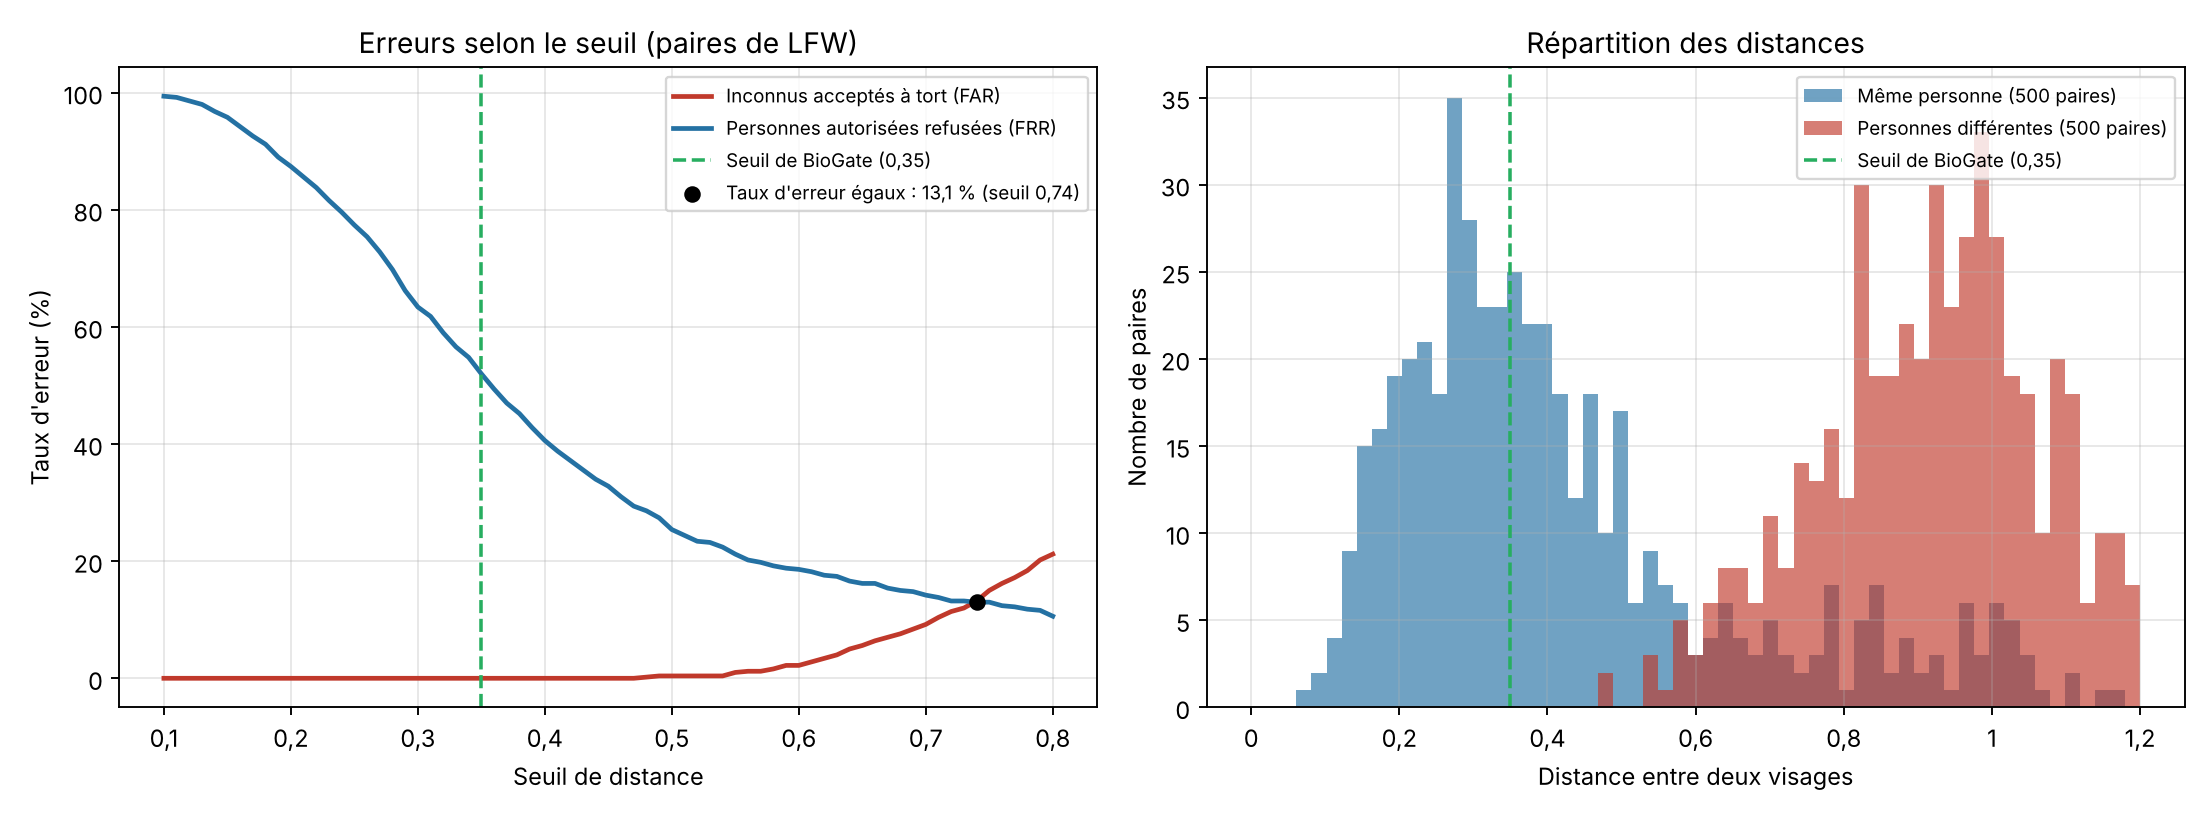
\includegraphics[width=\textwidth]{images/far_frr.png}
\caption{Taux d'erreur selon le seuil (à gauche) et distribution des distances (à droite), sur 1\,000 paires de LFW}\label{fig:farfrr}
\end{figure}

Le seuil de 0,35 est prudent : aucune fausse acceptation sur 500 paires, au prix de nombreux refus. Ces photographies sont prises dans des conditions non contrôlées, et chaque personne n'est comparée qu'à un seul échantillon. BioGate compare à plusieurs échantillons enrôlés à la webcam et retient le plus proche : son taux de faux rejet réel est donc plus bas que cette mesure, et son taux de fausse acceptation un peu plus haut. Aucune de ces deux valeurs n'a été mesurée pour BioGate en usage réel. L'écart avec les performances publiées pour FaceNet n'est pas expliqué : le détecteur, le recadrage ou le prétraitement peuvent y contribuer. Le seuil par défaut de DeepFace pour FaceNet512 est de 0,30 ; BioGate retient 0,35, valeur réglée à la webcam.

La mesure a deux limites : une seule série de 1\,000 paires, sans validation croisée sur les dix séries de LFW, et des photographies de personnalités, qui ne sont pas celles d'une caméra de porte. Le calcul des vecteurs a pris 635 secondes pour 1\,549 images, soit 0,41 seconde par image sur le processeur, détection de Haar et correction du contraste comprises.

\subsection{Reconnaissance en faible éclairage}

Le 2 novembre 2026, une séance a été observée sur le serveur réel avec une webcam peu éclairée, la luminosité moyenne de l'image étant de 49 sur 255. Le journal du serveur montre 39 reconfirmations du profil de l'auteur en 46 secondes, avec une distance moyenne de 0,178 (médiane de 0,160, minimum de 0,11, maximum de 0,29), toutes sous le seuil de 0,35, et un accès accordé avec un score de 75,2~\%. BioGate reconnaît donc l'auteur dans une pièce peu éclairée. Il s'agit d'une observation sur une séance et un visage, non d'une comparaison chiffrée avec un autre modèle.

\subsection{Qualité de la détection}

Des mesures sur des captures ont montré les limites d'un détecteur de personnes appliqué à des images en deux dimensions. À 320, 480 et 640 pixels, YOLOv8 nano attribue à une photographie de personne affichée sur un téléphone des confiances de 0,80, 0,85 et 0,86, et à une main placée près de l'objectif des confiances de 0,84, 0,89 et 0,71. Augmenter la résolution ne supprime donc pas la fausse détection, et aucun seuil de confiance ne sépare la photographie, à 0,80, d'une vraie silhouette partielle, à 0,37. Cette mesure a conduit à la règle selon laquelle un intrus est un visage inconnu, et non une silhouette sans visage.

Le détecteur de Haar a lui aussi produit une fausse détection : un pli de vêtement au niveau du col et d'un bouton d'une chemise a été pris pour un visage de 67 pixels, et une alerte avec la photo d'un torse a été envoyée par Telegram. Le second avis de MediaPipe rejette ce faux visage. Sur les images d'essai, la chemise est rejetée et les trois portraits de test sont acceptés. Cette validation repose sur une seule photographie de chemise et trois portraits, et non sur des visages de webcam sous des angles variés.

Avant les correctifs de la recette, le retour d'un individu classé intrus provisoire à l'état de résident prenait de 2 à 31 secondes, avec une médiane d'environ 15 secondes, sur 7 cas. Ce délai n'a pas été remesuré après la réanalyse patiente et la correspondance forte.

\subsection{Adaptation à l'évolution du visage}

L'essai d'adaptation suit un protocole en quatre étapes, sur une base de données isolée qui ne touche pas les profils réels :
\begin{enumerate}
  \item enrôlement d'un profil de référence avec une photographie \og avant \fg{} ;
  \item tentative de reconnaissance d'une photographie \og après \fg{}, avant tout apprentissage, pour établir que le problème existe ;
  \item simulation de l'apprentissage continu : le visage \og après \fg{} est ajouté au profil, comme le ferait une confirmation par empreinte ;
  \item nouvelle tentative sur une seconde photographie \og après \fg{}, différente de la première, pour vérifier que le système généralise.
\end{enumerate}

Le sujet est un acteur dont les photographies publiques, sous licence libre, couvrent onze ans et montrent à la fois le vieillissement et le passage d'un visage rasé à une barbe pleine (figure~\ref{fig:evans}). Ces images ne servent qu'à mesurer la distance entre deux vecteurs ; l'essai ne vise pas la personne photographiée.

\begin{figure}[H]
\centering
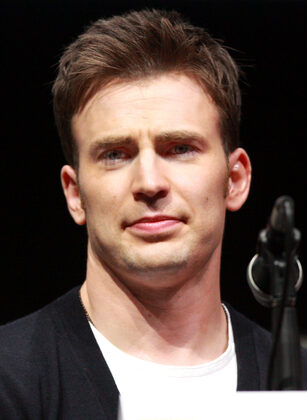
\includegraphics[width=0.30\textwidth]{images/evans_2013_Chris_Evans_rase.jpg}\hfill

\includegraphics[width=0.30\textwidth]{images/evans_2019_Chris_Evans_barbe.jpg}\hfill

\includegraphics[width=0.30\textwidth]{images/evans_2024_Chris_Evans_barbe.jpg}
\caption{Photographies de l'essai d'adaptation, de gauche à droite : 2013 (référence), 2019 (apprentissage) et 2024 (validation). Auteurs : Gage Skidmore, licence CC BY-SA~3.0~\cite{commons_evans_2013} ; Bureau du représentant Don Young, domaine public~\cite{commons_evans_2019} ; Amy Martin Photography, licence CC BY-SA~4.0~\cite{commons_evans_2024}. Source : Wikimedia Commons.}\label{fig:evans}
\end{figure}

Le tableau~\ref{tab:evans} donne les résultats, avec le seuil de reconnaissance de 0,35.

\begin{table}[H]
\centering
\caption{Résultat de l'essai d'adaptation}\label{tab:evans}
\small
\begin{tabularx}{\textwidth}{@{}>{\raggedright\arraybackslash}Xcc@{}}
\toprule
\textbf{Étape} & \textbf{Distance cosinus} & \textbf{Résultat} \\
\midrule
Avant apprentissage (photo de 2019 contre le profil de 2013) & 0,4722 & non reconnu \\
Après un apprentissage (photo de 2019 ajoutée), validation avec la photo de 2024 & 0,224 & reconnu \\
\bottomrule
\end{tabularx}
\end{table}

Le système échoue donc à reconnaître le sujet après le changement d'apparence tant qu'aucun apprentissage n'a eu lieu, et le reconnaît après une seule confirmation d'identité. La photographie de validation est différente de celle de l'apprentissage, ce qui écarte un simple rappel de l'image apprise. L'essai a toutefois une portée limitée : un seul sujet, un seul apprentissage, et une confirmation par empreinte simulée.

Une mesure contrôlée a ensuite été faite à la webcam sur le profil de l'auteur. Ce profil compte 8 vecteurs : l'enrôlement d'origine et sept vecteurs ajoutés par l'apprentissage continu. Pendant 40 secondes, le visage de face devant la caméra a donné 78 images retenues : la silhouette est trouvée par YOLO, le visage par Haar dans cette silhouette, puis confirmé par MediaPipe ; 9 faux visages ont été écartés. Pour les mêmes images, la distance au seul vecteur d'origine est comparée à la distance au plus proche des 8 vecteurs du profil. Le tableau~\ref{tab:webcam} donne les résultats.

\begin{table}[H]
\centering
\caption{Effet de l'apprentissage continu mesuré à la webcam (78 images)}\label{tab:webcam}
\small
\begin{tabularx}{\textwidth}{@{}>{\raggedright\arraybackslash}Xcc@{}}
\toprule
\textbf{Mesure} & \textbf{Vecteur d'origine seul} & \textbf{Profil complet (8 vecteurs)} \\
\midrule
Distance moyenne & 0,209 & 0,203 \\
Distance médiane & 0,206 & 0,204 \\
Écart-type & 0,044 & 0,027 \\
Pire image & 0,436 & 0,273 \\
Images sous le seuil de 0,35 & 76 sur 78 & 78 sur 78 \\
\bottomrule
\end{tabularx}
\end{table}

Pour un visage proche de son enrôlement, l'apprentissage supprime donc les pires cas, les deux images qui dépassaient le seuil, mais ne baisse presque pas la distance moyenne. La marge face à l'autre profil enrôlé reste positive pour toutes les images, avec un minimum de 0,109. Cette mesure a des limites : une personne, une séance, un seul éclairage, et des images consécutives très proches les unes des autres. Prendre le minimum sur plusieurs vecteurs baisse en outre mécaniquement la distance : la mesure montre l'ampleur de cet effet sur ce visage, non une meilleure reconnaissance en toutes conditions. Il s'agit d'une première lecture, faite de nuit. \adonner{Seconde lecture en pleine lumière à ajouter, avec le même script}

Le journal du serveur contenait par ailleurs deux moyennes de distance, 0,269 puis 0,106, relevées lors de deux séances de la recette du 29 octobre, avant et après quatre validations d'empreinte. La mesure contrôlée ne les reproduit pas : elles viennent de séances aux conditions différentes, et elles ne sont pas retenues comme effet de l'apprentissage.

\subsection{Test de vivacité}

Deux séances de la webcam ont été enregistrées le 13 juillet 2026 afin de calibrer les seuils du test de vivacité. La première compte 1\,606 images, avec 25 clignements et 14 sourires détectés, la seconde 3\,367 images, avec 25 clignements et 80 sourires. Les pics du coefficient de sourire atteignent de 0,60 à 0,75, ce qui a conduit à abaisser le seuil du sourire de 0,45 à 0,40 en conservant une marge. Le seuil du clignement est de 0,35.

Ces enregistrements servent au réglage des seuils. Ils ne mesurent pas la résistance du test à une attaque : aucune photographie, vidéo rejouée ou masque n'a été présentée au système, et l'efficacité de la protection reste à établir.

\subsection{Purge des photos}

La durée de conservation de 72 heures prévue au cahier des charges n'était pas appliquée. Au moment de la vérification, 41 photos d'intrus de 107 à 128 jours d'âge se trouvaient sur le disque, et même la purge manuelle ne pouvait pas les atteindre, car elles n'étaient rattachées à aucune ligne du journal. La purge est devenue automatique : elle s'exécute au démarrage du serveur, ce qui rattrape un arrêt prolongé, puis toutes les heures. Elle supprime les photos expirées et orphelines, et conserve les lignes du journal. L'heure de coupure est calculée par SQLite en temps universel, car un calcul en heure locale pouvait supprimer un événement tout neuf. Vingt-cinq tests vérifient ce comportement. La suppression des 41 photos n'a pas été constatée sur le serveur réel, qui avait été démarré avant la correction.

\subsection{Résilience}

La résilience a été éprouvée sur trois points :
\begin{itemize}
  \item \textbf{Caméra} : la carte se reconnecte seule au dernier réseau enregistré après un redémarrage. Lors d'un essai, elle a redémarré pendant que BioGate lisait son flux. La connexion s'est rétablie sans intervention, avec la même adresse, et le flux est revenu. La durée de la coupure n'a pas été mesurée ;
  \item \textbf{Serveur} : il rouvre une source vidéo perdue ;
  \item \textbf{Alertes} : l'envoi par Telegram a été testé en conditions réelles, avec réception de la photo de l'individu sur le téléphone, et la suppression d'un message de test a été vérifiée.
\end{itemize}
En revanche, l'envoi par courrier électronique n'a été vérifié qu'avec un serveur simulé. La reprise après une coupure provoquée du Wi-Fi et le comportement face à une coupure d'électricité n'ont pas été éprouvés.

\subsection{Synthèse des résultats}

Le tableau~\ref{tab:synthese} résume les mesures et leur portée.

\begin{table}[H]
\centering
\caption{Synthèse des résultats}\label{tab:synthese}
\small
\begin{tabularx}{\textwidth}{@{}>{\raggedright\arraybackslash}p{3.1cm}>{\raggedright\arraybackslash}X>{\raggedright\arraybackslash}p{4.3cm}@{}}
\toprule
\textbf{Domaine} & \textbf{Résultat} & \textbf{Portée} \\
\midrule
Détection & 15,2 images par seconde (YOLOv8 nano, processeur seul) & Un ordinateur, 1\,800 images \\
Taux d'erreur (LFW) & FAR de 0,0~\% et FRR de 52,0~\% au seuil de 0,35 ; point d'égal taux d'erreur de 13,1~\% & 1\,000 paires, un seul échantillon par personne \\
Filtre de visage & Gain de 48 à 78~\% sur la route d'analyse & Une photo, un processeur \\
Adaptation & Distance de 0,4722 à 0,224 après un apprentissage & Un sujet, empreinte simulée \\
Adaptation (webcam) & Moyenne de 0,209 à 0,203 ; pire image de 0,436 à 0,273 ; images au-dessus du seuil : 2 sur 78, puis aucune & Une personne, une séance, première lecture de nuit \\
Faible éclairage & 39 reconfirmations, distance moyenne de 0,178, toutes sous 0,35 & Une séance, un visage \\
Vivacité & Seuils calibrés sur 2 séances (4\,973 images) & Pas d'essai d'attaque \\
Purge des photos & Automatique, 25 tests & Non constatée sur le serveur réel \\
Caméra & Flux lu à 17 à 30 images par seconde, reconnexion au réseau enregistré & Une carte, coupure du Wi-Fi non provoquée \\
Alertes & Telegram reçu avec photo, suppression d'un message de test & Courrier non éprouvé en réel \\
\bottomrule
\end{tabularx}
\end{table}

\section{Discussion critique}

\subsection{Bilan}

L'objectif du travail était de réaliser un prototype de contrôle d'accès par reconnaissance faciale qui garde les données en local, résiste à la présentation d'une photographie et reste fiable malgré les changements d'apparence de ses utilisateurs. Le prototype réunit ces trois propriétés dans une même architecture, avec des réserves qu'il convient d'énoncer.

Premièrement, le traitement est local. L'analyse des images, le calcul des vecteurs, la base et la purge s'exécutent sur le serveur, et le fonctionnement de base n'appelle aucun service extérieur : seuls les envois d'alerte sortent du système, et ils sont désactivés tant que le propriétaire ne les active pas. La photographie de l'intrus transite toutefois par Telegram, et le message est supprimé de la conversation après 24 heures.

Deuxièmement, un test de vivacité actif est en place. Il tire au sort un geste à chaque tentative et il a été calibré sur des enregistrements réels. Son efficacité contre des attaques n'a pas été mesurée, et le prototype ne dispose que d'une caméra à deux dimensions.

Troisièmement, l'adaptation aux changements d'apparence fonctionne selon l'essai mené : un apprentissage confirmé par un second facteur suffit à faire reconnaître un sujet dont l'apparence a changé. L'essai porte cependant sur un sujet et une confirmation simulée, et l'adaptation n'a lieu que si le second facteur est exigé. Une mesure à la webcam sur le profil de l'auteur montre que l'apprentissage supprime les pires cas sans baisser beaucoup la distance moyenne.

Enfin, la mesure sur 1\,000 paires de LFW donne, au seuil retenu, aucune fausse acceptation et 52~\% de faux rejets avec un seul échantillon par personne. Le seuil est prudent, et le taux de faux rejet de BioGate en usage réel n'est pas mesuré.

Par ailleurs, le travail a permis de mettre au jour des défauts qu'aucun test existant ne détectait, ce qui montre l'intérêt de la recette en conditions réelles.

\subsection{Défauts découverts et corrigés}

Le tableau~\ref{tab:defauts} recense les défauts relevés au fil du développement, leur cause et leur correction.

\begin{table}[H]
\centering
\caption{Défauts découverts et corrigés}\label{tab:defauts}
\small
\begin{tabularx}{\textwidth}{@{}>{\raggedright\arraybackslash}p{3.3cm}>{\raggedright\arraybackslash}X>{\raggedright\arraybackslash}X@{}}
\toprule
\textbf{Défaut} & \textbf{Cause} & \textbf{Correction} \\
\midrule
Journal illisible (erreur du serveur) & Scores stockés au format binaire de la bibliothèque numérique ; 203 lignes corrompues & Conversion en nombre simple, lignes réparées \\
Alertes sans photo & La photo n'était jamais rattachée à l'intrus & Rattachement à l'intrus provisoire, jamais à un résident \\
Photos hors de portée de la purge & Fichier sans ligne de journal quand le résident revient ou que la personne s'éloigne & Suppression dans ces deux cas \\
Purge jamais appliquée & Purge seulement manuelle ; 41 photos de 107 à 128 jours & Purge automatique au démarrage puis toutes les heures \\
Inconnus sans cadre à l'écran & Erreur avalée, 996 avertissements en deux minutes & Correction et test de non-régression \\
Faux intrus sur une main ou un torse & Détecteur de personnes trompé par des images partielles & Un intrus est un visage inconnu \\
Faux visage sur une chemise & Détecteur de Haar sur un col et un bouton & Second avis de MediaPipe \\
Noms d'intrus dupliqués & Compteur remis à zéro au rechargement des vecteurs & Compteur qui ne recule jamais \\
Détection de Haar en double & Seconde détection pour dessiner l'encadré & Réutilisation de la position mémorisée \\
Routes sans jeton (configuration, actionneurs) & Oubli de la vérification & Jeton exigé sur ces routes \\
Réglage de vivacité sans effet & Les deux pipelines ne lisaient pas le réglage & Règle commune et 8 tests \\
Redémarrage de la carte toutes les 30 secondes & Chien de garde de 20 secondes armé avant la connexion Wi-Fi et l'initialisation de la caméra & Chien de garde supprimé, aucune coupure sur 87 secondes ensuite \\
Aucune image lue par OpenCV & La ligne de séparation du flux doit précéder la première image, l'exemple du fabricant ne l'envoie qu'après & Ligne envoyée avant la première image, avec test de contre-épreuve \\
Carte bloquée après le départ d'un client & La fonction d'écriture de la bibliothèque est déclarée booléenne mais renvoie $-1$ en cas d'échec, que rien ne détecte & Délai de réception court et lecture d'un octet par image \\
Première requête lente après un repos & Économie d'énergie du Wi-Fi, de 7 à 27 secondes & Économie d'énergie désactivée \\
Messages d'alerte conservés chez le fournisseur & La purge ne concernait que le disque du serveur & Suppression des messages après 24 heures \\
Second avis de MediaPipe absent sur une copie propre & Le fichier du modèle est ignoré par git et rien ne le téléchargeait & Script de téléchargement avec empreinte SHA-256, étape dans la procédure d'installation, 5 tests \\
Installation non reproductible & Deux paquets OpenCV de versions différentes pour le même dossier de programmes & Les deux paquets fixés à la même version, versions des bibliothèques fixées, vérification dans un environnement neuf \\
Libellés des profils faux au tableau de bord & Libellé non aligné sur le comportement du serveur & Libellés des profils bureau et haute sécurité corrigés \\
\bottomrule
\end{tabularx}
\end{table}

Un enseignement général s'en dégage : aucun des tests existants n'avait vu le défaut des inconnus sans cadre, parce qu'aucun n'exécutait le pipeline multi-caméras avec une personne inconnue. Il a fallu un essai réel et la lecture du journal du serveur, qui est devenu un outil de validation à part entière.

\subsection{Limites observées}

Les limites du prototype sont les suivantes :
\begin{itemize}
  \item \textbf{Périmètre de validation} : l'évaluation est exploratoire ; les taux d'erreur reposent sur une seule série de 1\,000 paires de LFW, et non sur une caméra de porte, et les autres essais portent sur peu de personnes et de photographies ;
  \item \textbf{Efficacité anti-usurpation} : aucune attaque par photographie, vidéo rejouée ou masque n'a été présentée, et la caméra ne mesure pas la profondeur ;
  \item \textbf{Matériel simulé} : le lecteur d'empreinte, la gâche et la lumière sont simulés, et l'écran LCD des consignes, reporté à la fin du projet, n'est pas réalisé ;
  \item \textbf{Portage} : l'exécution sur un micro-ordinateur monocarte de type Raspberry Pi est visée mais n'a pas été essayée, et la quantification des modèles n'est pas faite ;
  \item \textbf{Visages proches} : deux profils de résidents ont des visages proches : le vecteur du second profil le plus proche du profil principal est à 0,306, sous le seuil de 0,35, et une confusion est possible. En direct, des distances de 0,23 à 0,35 ont été observées entre le visage de l'auteur et ce second profil. La mesure à la webcam donne une marge toujours positive entre les deux profils, d'au moins 0,109. Aucune marge de décision entre profils proches n'est ajoutée, et ce cas est exclu des essais finaux ;
  \item \textbf{Caméra} : la clé du flux et le réseau Wi-Fi sont mémorisés sans chiffrement dans la mémoire flash de la carte, et la reprise après une coupure provoquée du Wi-Fi n'a pas été éprouvée ;
  \item \textbf{Sources vidéo} : le flux RTSP n'a pas été vérifié, faute de serveur RTSP, ni le HTTPS ;
  \item \textbf{Sécurité des échanges} : pas de HTTPS, onze routes sans jeton dont celles utilisées par l'outil de développement, et aucun audit de sécurité externe ;
  \item \textbf{Protection des données} : les vecteurs ne sont pas chiffrés dans la base, les identifiants des canaux d'alerte y sont enregistrés en clair, et la table d'audit prévue n'est pas implémentée ;
  \item \textbf{Messages Telegram} : les messages envoyés avant la suppression automatique restent dans la conversation, et la suppression d'une alerte accompagnée d'une photo n'a pas été essayée en conditions réelles ;
  \item \textbf{Journal} : les lignes du journal ne sont pas purgées, seules les photos le sont ;
  \item \textbf{Alertes} : un envoi qui échoue n'est pas renvoyé, un intrus qui quitte le champ avant la fin de la fenêtre de grâce n'est pas signalé, et un passant sans visage ne déclenche aucune alerte à distance ;
  \item \textbf{Réglages} : la durée d'analyse et l'intervalle de revérification ne prennent effet qu'au redémarrage du serveur ;
  \item \textbf{Alimentation} : une coupure d'électricité arrête le serveur et fait perdre les états en mémoire, dont le jeton du tableau de bord.
\end{itemize}
Ces limites ne remettent pas en cause l'intérêt de l'approche. Elles précisent ce qu'il reste à faire pour passer du prototype à un produit.

\section{Perspectives}

Les suites du travail s'articulent autour des axes suivants :
\begin{itemize}
  \item \textbf{Sécuriser les échanges} : étendre le jeton à toutes les routes, ajouter une authentification des équipements, passer en HTTPS et faire réaliser un audit externe ;
  \item \textbf{Protéger les données} : chiffrer les vecteurs et les identifiants dans la base ainsi que les réglages mémorisés dans la carte, et ne conserver que des gabarits chiffrés, comme l'impose, sur les lieux de travail, le règlement type de la CNIL pris ici comme référence~\cite{cnil2019reglementtype} ;
  \item \textbf{Compléter le matériel} : relier un lecteur d'empreinte et une gâche réels, réaliser l'écran LCD des consignes, et ajouter des modules d'autonomie pour supporter les coupures de courant ;
  \item \textbf{Renforcer l'anti-usurpation} : ajouter un capteur de profondeur et mesurer la résistance du test de vivacité selon la norme ISO/IEC 30107-3~\cite{iso30107} ;
  \item \textbf{Évaluer à plus grande échelle} : valider la mesure des taux d'erreur sur les dix séries de LFW, puis avec plusieurs échantillons par personne enrôlés à la webcam ;
  \item \textbf{Élargir les alertes} : valider l'envoi par courrier électronique avec un vrai serveur, essayer en conditions réelles la suppression d'une alerte accompagnée d'une photo, et envisager WhatsApp malgré son coût par message ;
  \item \textbf{Alléger le calcul} : quantifier les modèles et porter le système sur un micro-ordinateur monocarte ;
  \item \textbf{Respecter le cadre légal} : accomplir les formalités auprès de l'Autorité de protection des données à caractère personnel et recueillir le consentement explicite des personnes enrôlées, comme l'exige le Code du numérique béninois.
\end{itemize}

\addcontentsline{toc}{section}{Conclusion}
\section*{Conclusion}

Ce chapitre a présenté l'implémentation de BioGate, les essais menés et leurs enseignements. Le prototype fonctionne de bout en bout : la caméra alimente le serveur, qui détecte, suit et reconnaît les personnes, demande un second facteur si nécessaire et envoie une alerte par Telegram en cas d'intrusion. Les essais montrent que l'adaptation du profil à un changement d'apparence est possible, que la détection est assez rapide pour un usage domestique sur un simple processeur et que la purge des photos est automatisée. Ils montrent aussi les limites du travail : une évaluation exploratoire, un matériel en partie simulé et une sécurité à renforcer avant tout déploiement. Ces limites constituent les axes de poursuite présentés dans les perspectives.


% \include{perspectives}
%%conclusion
\conclusion
Ce travail a porté sur la conception et la réalisation de BioGate, un prototype de contrôle d'accès par reconnaissance faciale qui traite les données en local, vérifie la présence réelle de la personne et s'adapte à l'évolution de son visage. Les solutions existantes réunissent rarement ces trois propriétés : les caméras reliées à un service en ligne confient les images à un tiers et reposent sur un abonnement, tandis que la solution qui les réunit, Face ID, est propriétaire et propre aux appareils d'un seul fabricant. L'objectif était de les rassembler dans une architecture modulaire, utilisable sans abonnement ni connexion Internet pour son fonctionnement de base.

Le prototype réalisé détecte et suit les personnes devant la caméra, filtre les visages de face, calcule pour chacun un vecteur de 512 nombres et le compare aux profils enrôlés. Un score de confiance et un second facteur, l'empreinte ou un geste tiré au sort, encadrent l'accès. Les photos des individus soupçonnés sont purgées automatiquement et le propriétaire est alerté par Telegram. Un tableau de bord permet de superviser le système et de régler son comportement. Les essais montrent qu'une seule confirmation d'identité suffit à faire reconnaître un sujet dont l'apparence a changé : la distance mesurée passe de 0,4722 à 0,224, sous le seuil de reconnaissance de 0,35. Ils montrent aussi que le traitement reste assez rapide pour un usage domestique sur un simple processeur. Sur 1\,000 paires de la base LFW, le seuil retenu n'accepte aucun inconnu et refuse 52~\% des paires d'une même personne comparées à un seul échantillon, mesure qui ne donne pas le taux de faux rejet de BioGate en usage réel.

Certaines limites subsistent néanmoins. L'évaluation est exploratoire, le lecteur d'empreinte et les actionneurs sont simulés, l'efficacité du test de vivacité contre des attaques n'a pas été mesurée, et la sécurité des échanges et des données doit être renforcée avant tout déploiement. Ces limites constituent des axes d'amélioration pour les versions futures.

Les perspectives d'évolution de BioGate s'articulent autour des axes suivants :
\begin{itemize}
  \item sécuriser les échanges et chiffrer les données biométriques, afin de répondre aux exigences de protection des données personnelles ;
  \item compléter le matériel avec un lecteur d'empreinte, une gâche et un capteur de profondeur, puis mesurer la résistance du test de vivacité aux attaques par photographie, vidéo et masque ;
  \item évaluer le système sur un plus grand nombre de personnes et le porter sur un micro-ordinateur monocarte.
\end{itemize}

En définitive, BioGate montre qu'il est possible de réunir traitement local, vérification de la présence et adaptation du visage dans un même prototype, tout en précisant ce qu'il reste à établir par des mesures à plus grande échelle.

%
\lhead[]{} \rhead[]{} \chead[]{}

%%biblio
\addcontentsline{toc}{chapter}{Bibliographie}
\bibliographystyle{abbrv}
\bibliography{biblio}


%\chapter*{Annexe}\addcontentsline{toc}{chapter}{Annexe}\label{annexe1}

\subsection*{Étapes clés du déroulement de l'attaque}


Nous allons exploiter quelques failles de ce réseau pour effectuer une attaque man in the middle (MITM).\\

Au début, notre machine Windows peut atteindre normalement le routeur R4.
\begin{figure}[H]
    \centering
    \includegraphics[scale=0.8]{images/ping_b4_1}
    \caption{Ping vers le routeur R4 avec succès}
    \label{fig:ping_b4_1}
\end{figure}
Quand on essaie de tracer le chemin vers R4, on constate que la machine passe par le routeur R1 légitime du lien pour atteindre R4
\begin{figure}[H]
    \centering
    \includegraphics{images/tracert_b4_1}
    \caption{Traces du chemin vers R4}
    \label{fig:tracert_b41}
\end{figure}
L'attaquant sur le lien peut alors passer a l'attaque.
Pour effectuer l'attaque MITM on utilisera l'outil fake\_router6, un utilitaire du package d'outils \textbf{the hacker choice}.
Ainsi sur la machine d'attaque, on active en un premier lieu le forwarding pour être transparent et ne pas bloquer le transit des paquets.
\begin{figure}[H]
    \centering
    \includegraphics{images/attk/fwrd_activation}
    \caption{Activation du forwarding des paquets.}
    \label{fig:activ_fwrd}
\end{figure}
Aussi on lance wireshark pour observer le trafic des paquets sur notre interface dans le réseau.\\
-------\\
Puisque tout est prêt nous allons lancer l'attaque.

\begin{figure}[H]
    \centering
    \includegraphics[scale=0.8]{images/attk/lancement_attk_1}
    \caption{Initialisation de l'attaque}
    \label{fig:attk_init_1}
\end{figure}

L'attaque est en cours et l'attaquant s'annonce comme le routeur par défaut du lien
nous allons maintenant vérifier la table des routes de notre machine windows.
\begin{figure}[H]
    \centering
    \includegraphics{images/attk/tableRoutes_windows}
    \caption{Table des routes de la machine victime}
    \label{fig:win_route_table}
\end{figure}
On constate que l'attaquant s'est insère comme passerelle de la victime.
pour confirmer cela reprenons un tracert vers le routeur r4
\begin{figure}[H]
    \centering
    \includegraphics{images/attk/tracert_b4_2}
    \caption{Chemin vers b4 pendant l'attaque.}
    \label{fig:tracert_b42}
\end{figure}
On peut voir clairement que la victime passe par l'attaquant pour atteindre le routeur.\\

A présent nous allons essayer de capturer une information envoyée par la victime.
Pour cela la victime fait un telnet sur le router R4 pour s'y connecter avec les paramètres suivants:\\
password1:\textbf{cisco}\\
password2:\textbf{class}
\begin{figure}[H]
    \centering
    \includegraphics{images/attk/telnet_r4}
    \caption{Connexion telnet au routeur.}
    \label{fig:telnetr4}
\end{figure}

Une fois la connexion réussie, nous allons voir avec wireshark les paquets de connexion et y retrouver les paramètres de connexion.
\begin{figure}[H]
    \centering
    \includegraphics[width=1.0\textwidth]{images/attk/c}
    \includegraphics[width=1.0\textwidth]{images/attk/i}
    \includegraphics[width=1.0\textwidth]{images/attk/s}
    \includegraphics[width=1.0\textwidth]{images/attk/c2}
    \includegraphics[width=1.0\textwidth]{images/attk/o}   
    \caption{Premier paramètre de connexion au routeur R4: \textbf{c-i-s-c-o}}
    \label{fig:param_conn_r4}
\end{figure}
\begin{figure}[H]
    \centering
    \includegraphics[width=1.0\textwidth]{images/attk/param2_c}
    \includegraphics[width=1.0\textwidth]{images/attk/param2_l}
    \includegraphics[width=1.0\textwidth]{images/attk/param2_a}
    \includegraphics[width=1.0\textwidth]{images/attk/param2_s1}
    \includegraphics[width=1.0\textwidth]{images/attk/param2_s2}
    \caption{Second paramètre de connexion au routeur R4: \textbf{c-l-a-s-s}}
    \label{fig:param_conn2}
\end{figure}
Les paramètres on été retrouves donc l'attaque a été un succès!

%\subsection*{Mitigations}
%Pour sécuriser ce réseau afin d'éviter ce genre d'attaque, deux mesures de sécurité peuvent être configurées.
%\begin{itemize}
%    \item le SEND
%    \item le RaGuard
%\end{itemize}



\newpage
\tableofcontents

\end{document}
